%%%%%%%%%%%%%%%%%%%%%%%%%%%%%%%%%%%%%%%%%
% Jacobs Landscape Poster
% LaTeX Template
% Version 1.1 (14/06/14)
%
% Created by:
% Computational Physics and Biophysics Group, Jacobs University
% https://teamwork.jacobs-university.de:8443/confluence/display/CoPandBiG/LaTeX+Poster
% 
% Further modified by:
% Nathaniel Johnston (nathaniel@njohnston.ca)
%
% This template has been downloaded from:
% http://www.LaTeXTemplates.com
%
% License:
% CC BY-NC-SA 3.0 (http://creativecommons.org/licenses/by-nc-sa/3.0/)
%
%%%%%%%%%%%%%%%%%%%%%%%%%%%%%%%%%%%%%%%%%

%----------------------------------------------------------------------------------------
%	PACKAGES AND OTHER DOCUMENT CONFIGURATIONS
%----------------------------------------------------------------------------------------

\documentclass[final]{beamer}

\usepackage[scale=0.9]{beamerposter} % Use the beamerposter package for laying out the poster
\usetheme{confposter} % Use the confposter theme supplied with this template

\setbeamercolor{block title}{fg=dblue!80,bg=white} % Colors of the block titles
\setbeamercolor{block body}{fg=black,bg=white} % Colors of the body of blocks
\setbeamercolor{block alerted title}{fg=white,bg=dblue!70} % Colors of the highlighted block titles
\setbeamercolor{block alerted body}{fg=black,bg=dblue!10} % Colors of the body of highlighted blocks
\setbeamertemplate{caption}[numbered]

% Many more colors are available for use in beamerthemeconfposter.sty

%-----------------------------------------------------------
% Define the column widths and overall poster size
% To set effective sepwid, onecolwid and twocolwid values, first choose how many columns you want and how much separation you want between columns
% In this template, the separation width chosen is 0.024 of the paper width and a 4-column layout
% onecolwid should therefore be (1-(# of columns+1)*sepwid)/# of columns e.g. (1-(4+1)*0.024)/4 = 0.22
% onecolwid should therefore be (1-(# of columns+1)*sepwid)/# of columns e.g. 
% (1-(3+1)*0.025)/3 = 0.3
% Set twocolwid to be (2*onecolwid)+sepwid = 0.464
% Set threecolwid to be (3*onecolwid)+2*sepwid = 0.708
\newcommand{\Cyclus}{\textsc{Cyclus}\xspace}%

\newlength{\sepwid}
\newlength{\onecolwid}
\newlength{\twocolwid}
\newlength{\threecolwid}
\setlength{\paperwidth}{33.1in} % A0 width: 46.8in
\setlength{\paperheight}{46.8in} % A0 height: 33.1in
\setlength{\textwidth}{33.1in} % A0 width: 46.8in
\setlength{\textheight}{46.8in} % A0 height: 33.1in
\setlength{\sepwid}{0.025\paperwidth} % Separation width (white space) between columns
\setlength{\onecolwid}{0.3\paperwidth} % Width of one column
\setlength{\twocolwid}{0.625\paperwidth} % Width of two columns
\setlength{\threecolwid}{0.95\paperwidth} % Width of three columns
\setlength{\topmargin}{-1in} % Reduce the top margin size
%-----------------------------------------------------------

\usepackage{graphicx}  % Required for including images
\usepackage{hyperref}
\usepackage{cite}


\usepackage{tabularx}
\newcolumntype{b}{X}
\newcolumntype{s}{>{\hsize=.5\hsize}X}
\newcolumntype{m}{>{\hsize=.75\hsize}X}
\newcolumntype{z}{>{\hsize=.65\hsize}X}

\usepackage{booktabs} % Top and bottom rules for tables
\usepackage{xspace}

\usepackage{tikz}
\usepackage{chronology}
\usetikzlibrary{arrows.meta}

\usetikzlibrary{positioning, arrows, decorations, shapes, calc }
% Define block styles
\tikzstyle{decision} = [diamond, draw, fill=blue!20, 
text width=4.5em, text badly centered, node distance=3cm, inner sep=0pt]

\tikzstyle{const} = [rectangle, draw, text centered, fill=orange!20]
\tikzstyle{data} = [rectangle, draw, text centered, fill=green!20]

\tikzstyle{block} = [rectangle, draw, text centered, fill=blue!20]
\tikzstyle{line} = [draw, -latex']
\tikzstyle{cloud} = [draw, ellipse,fill=red!20, node distance=6em,
minimum height=2em]



\usetikzlibrary{shapes.multipart}
\usetikzlibrary{positioning}


%-----------------------------------------------------------
% KNOWN ISSUE IN TIKZ MATH: tiny big symbols, like sum.
%-----------------------------------------------------------

% declare `cmex` to be arbitrary scalable
\DeclareFontShape{OMX}{cmex}{m}{n}{
  <-7.5> cmex7
  <7.5-8.5> cmex8
  <8.5-9.5> cmex9
  <9.5-> cmex10
}{}

\SetSymbolFont{largesymbols}{normal}{OMX}{cmex}{m}{n}
\SetSymbolFont{largesymbols}{bold}  {OMX}{cmex}{m}{n}

\usepackage{amssymb}
\usepackage{pifont}
\usepackage{xcolor}
\newcommand{\greencheck}{{\color{green}\checkmark}}
\newcommand{\xmark}{{\color{red}\ding{55}}}

\setbeamertemplate{bibliography item}[text]

\makeatletter
\def\beamer@andinst{\\[0em]}
\makeatother


%----------------------------------------------------------------------------------------
%	TITLE SECTION 
%----------------------------------------------------------------------------------------

\title{Dynamic Transition Analysis with TIMES}

\author{
       % \textbf{ENERGY ANALYSIS DIVISION}\\
       % \textbf{I\textsuperscript{2}CNER Initiative on Challenges in Energy Assessment and Energy Transitions}\\
        Anshuman Chaube\inst{1}, Andrew Chapman\inst{2}, James Stubbins\inst{1}, \textbf{Kathryn Huff}\inst{1}}
\institute[shortinst]{ \inst{1} University of Illinois at Urbana-Champaign, Department of Nuclear, Plasma, and Radiological Engineering, Urbana, USA \and \inst{2} International Institute for Carbon Neutral Energy Research (I$^2$CNER), Kyushu University, Fukuoka, Japan}
%----------------------------------------------------------------------------------------

\begin{document}

\addtobeamertemplate{block end}{}{\vspace*{2ex}} % White space under blocks
\addtobeamertemplate{block alerted end}{}{\vspace*{2ex}} % White space under highlighted (alert) blocks

\setlength{\belowcaptionskip}{2ex} % White space under figures
\setlength\belowdisplayshortskip{2ex} % White space under equations

\begin{frame}[t] % The whole poster is enclosed in one beamer frame

\begin{columns}[t,totalwidth=\threecolwid] % The whole poster consists of three major columns, the second of which is split into two columns twice - the [t] option aligns each column's content to the top


%=======================================================
% FIRST COLUMN BEGINS
%=========================================================


\begin{column}{\twocolwid} % The first two columns, two cols wide
\begin{columns}[t,totalwidth=\twocolwid] % Split up the first column into two, 
\begin{column}{\onecolwid} % The first column, one col wide

%----------------------------------------------------------------------------------------
%	OBJECTIVES
%----------------------------------------------------------------------------------------

\begin{alertblock}{Objectives}

\begin{description}
{%\large 
        \item[\textbf{Division:}] Energy Analysis Division
        \item[\textbf{Project:}] I\textsuperscript{2}CNER Initiative on Challenges in Energy Assessment and Energy Transitions
        \item[\textbf{Objective:}] Evaluate potential impact of novel energy technologies within Japan's energy system.
\item[\textbf{Milestones:}] ~\\}
        \begin{itemize}
        \item Minimize carbon emissions within realistic constraints.
        \item Create realistic decarbonization roadmaps.
	    \item Identify high impact technologies.
        \item Identify potential transition bottlenecks.
        %\item Help create timelines for R\&D investment and infrastructure development.
     	\end{itemize}
\end{description}

\end{alertblock}
%
%\begin{block}{Collaborators}
%
%I\textsuperscript{2}CNER collaborators will include primarily the members of 
%the Energy Analysis Division (EAD), including those members at other 
%institutes, universities or industries with connections to the EAD.   
%\end{block}

%----------------------------------------------------------------------------------------
%	METHODOLOGY
%----------------------------------------------------------------------------------------

\begin{block}{Introduction}
Previous work has compared the impact of innovative energy technologies in 
various world regions using \textbf{static} scenario analyses 
\cite{kikuchi_simulation-based_2017,pambudi_impact_2017}.  
We are simulating \textbf{dynamic} transition scenarios 
\cite{pfenninger_energy_2014} aimed at \textbf{optimizing energy supply} to minimize carbon 
emissions in Japan to 80\% of 1990 levels by 2050.
Our model has conventional and I$^2$CNER technologies (\textbf{carbon capture(CCS)} \& \textbf{H$_2$} production).
\end{block}

%\vspace{77mm}

\begin{figure}[H] 
\centering

\includegraphics[scale=1.1]{legend}
%\caption{Legend}
\label{legend}
\end{figure}

\begin{figure}[H] 
\centering
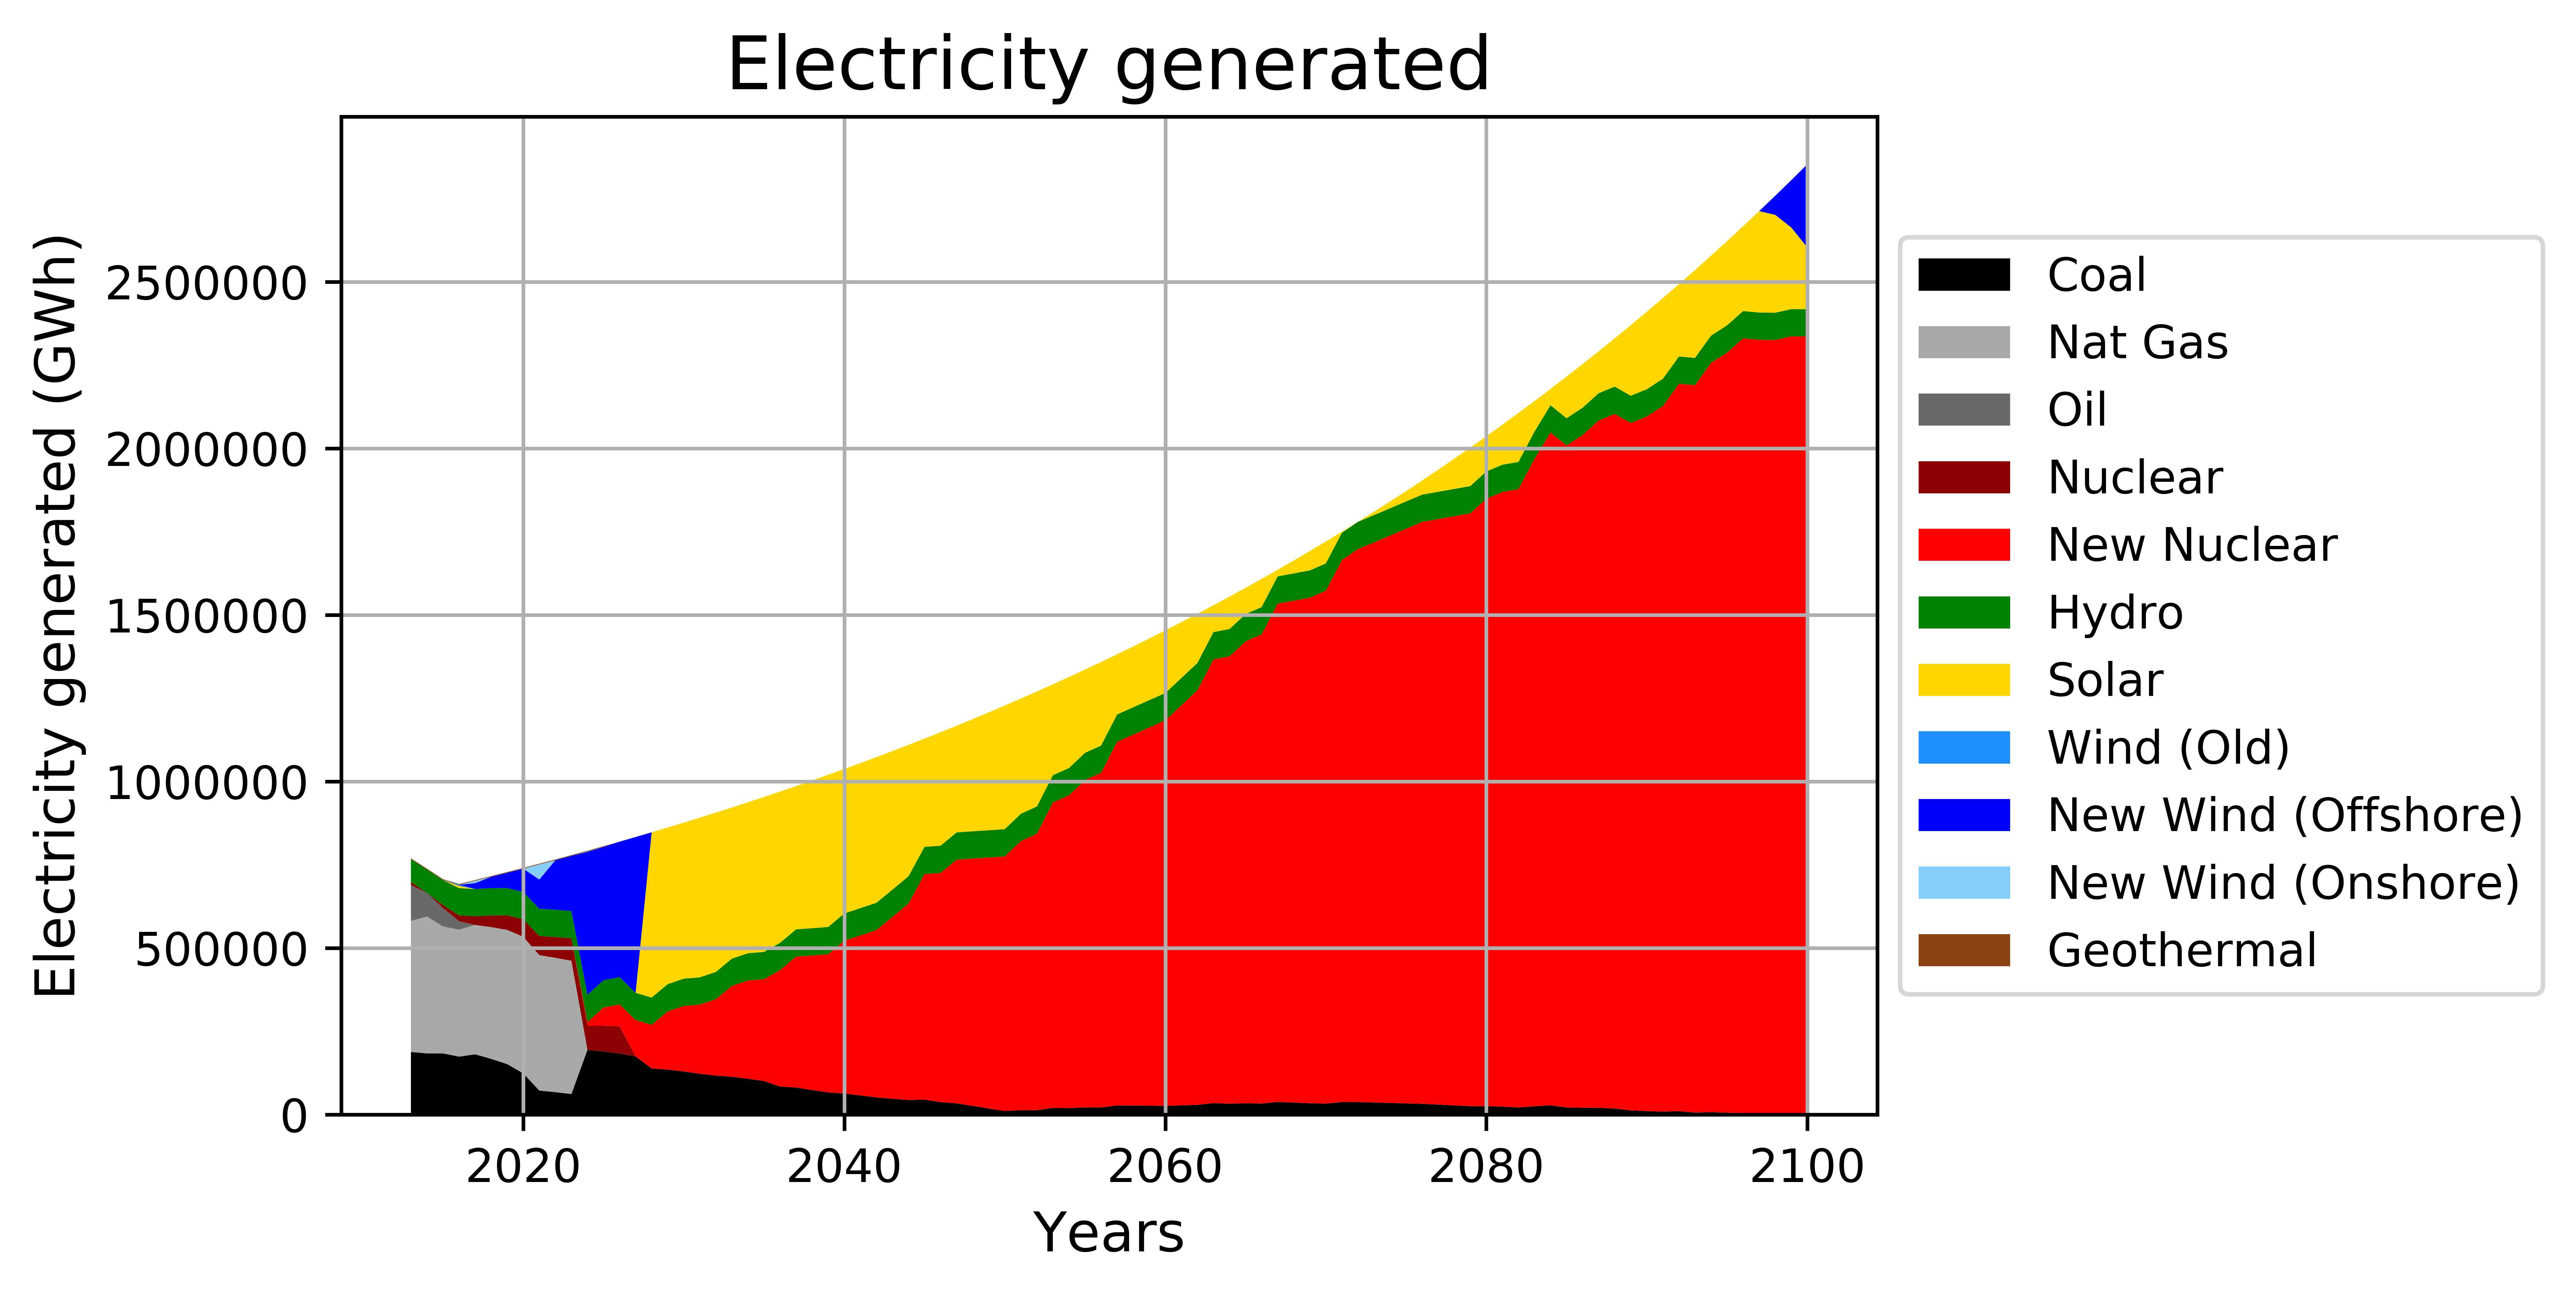
\includegraphics[scale=1.51]{conv_nuc_elc}
\caption{\textbf{Scenario 1} (conventional, with new nuclear) Electricity Generation.}
\label{s1e}
\end{figure}

\begin{figure}[H] 
\centering
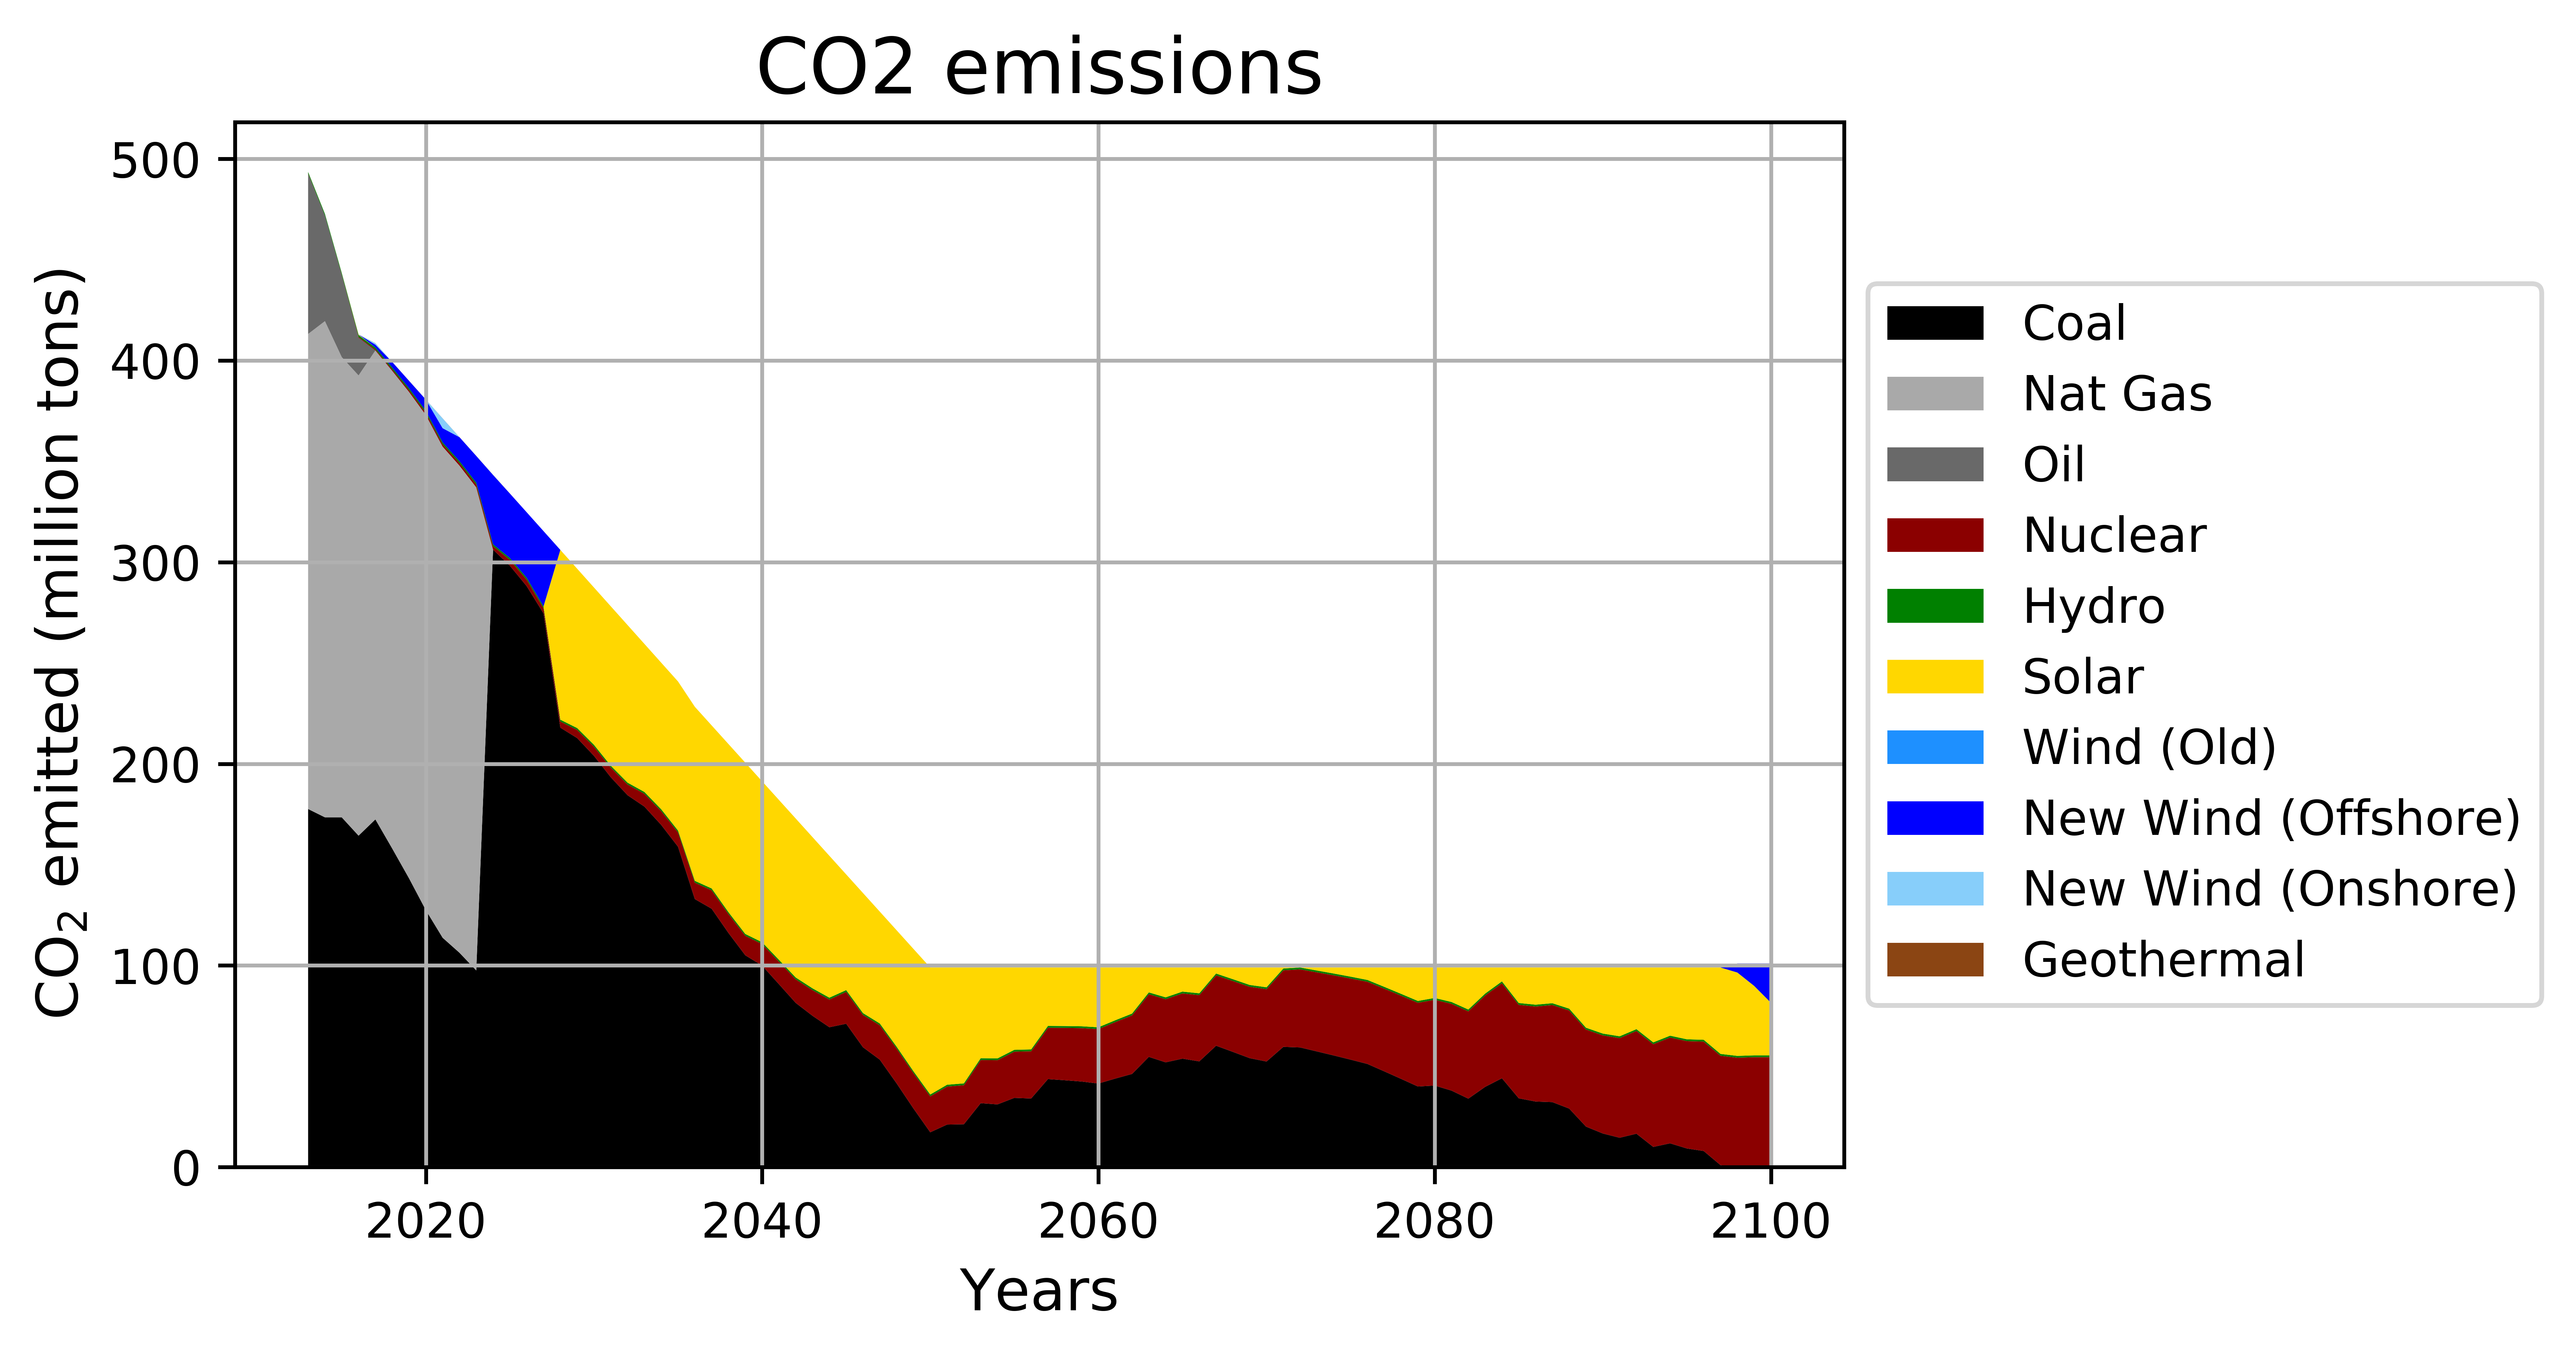
\includegraphics[scale=1.51]{conv_nuc_co2}
\caption{\textbf{Scenario 1} (conventional, with new nuclear) CO$_2$ emissions.}
\label{s1c}
\end{figure}


\begin{figure}[H] 
\centering
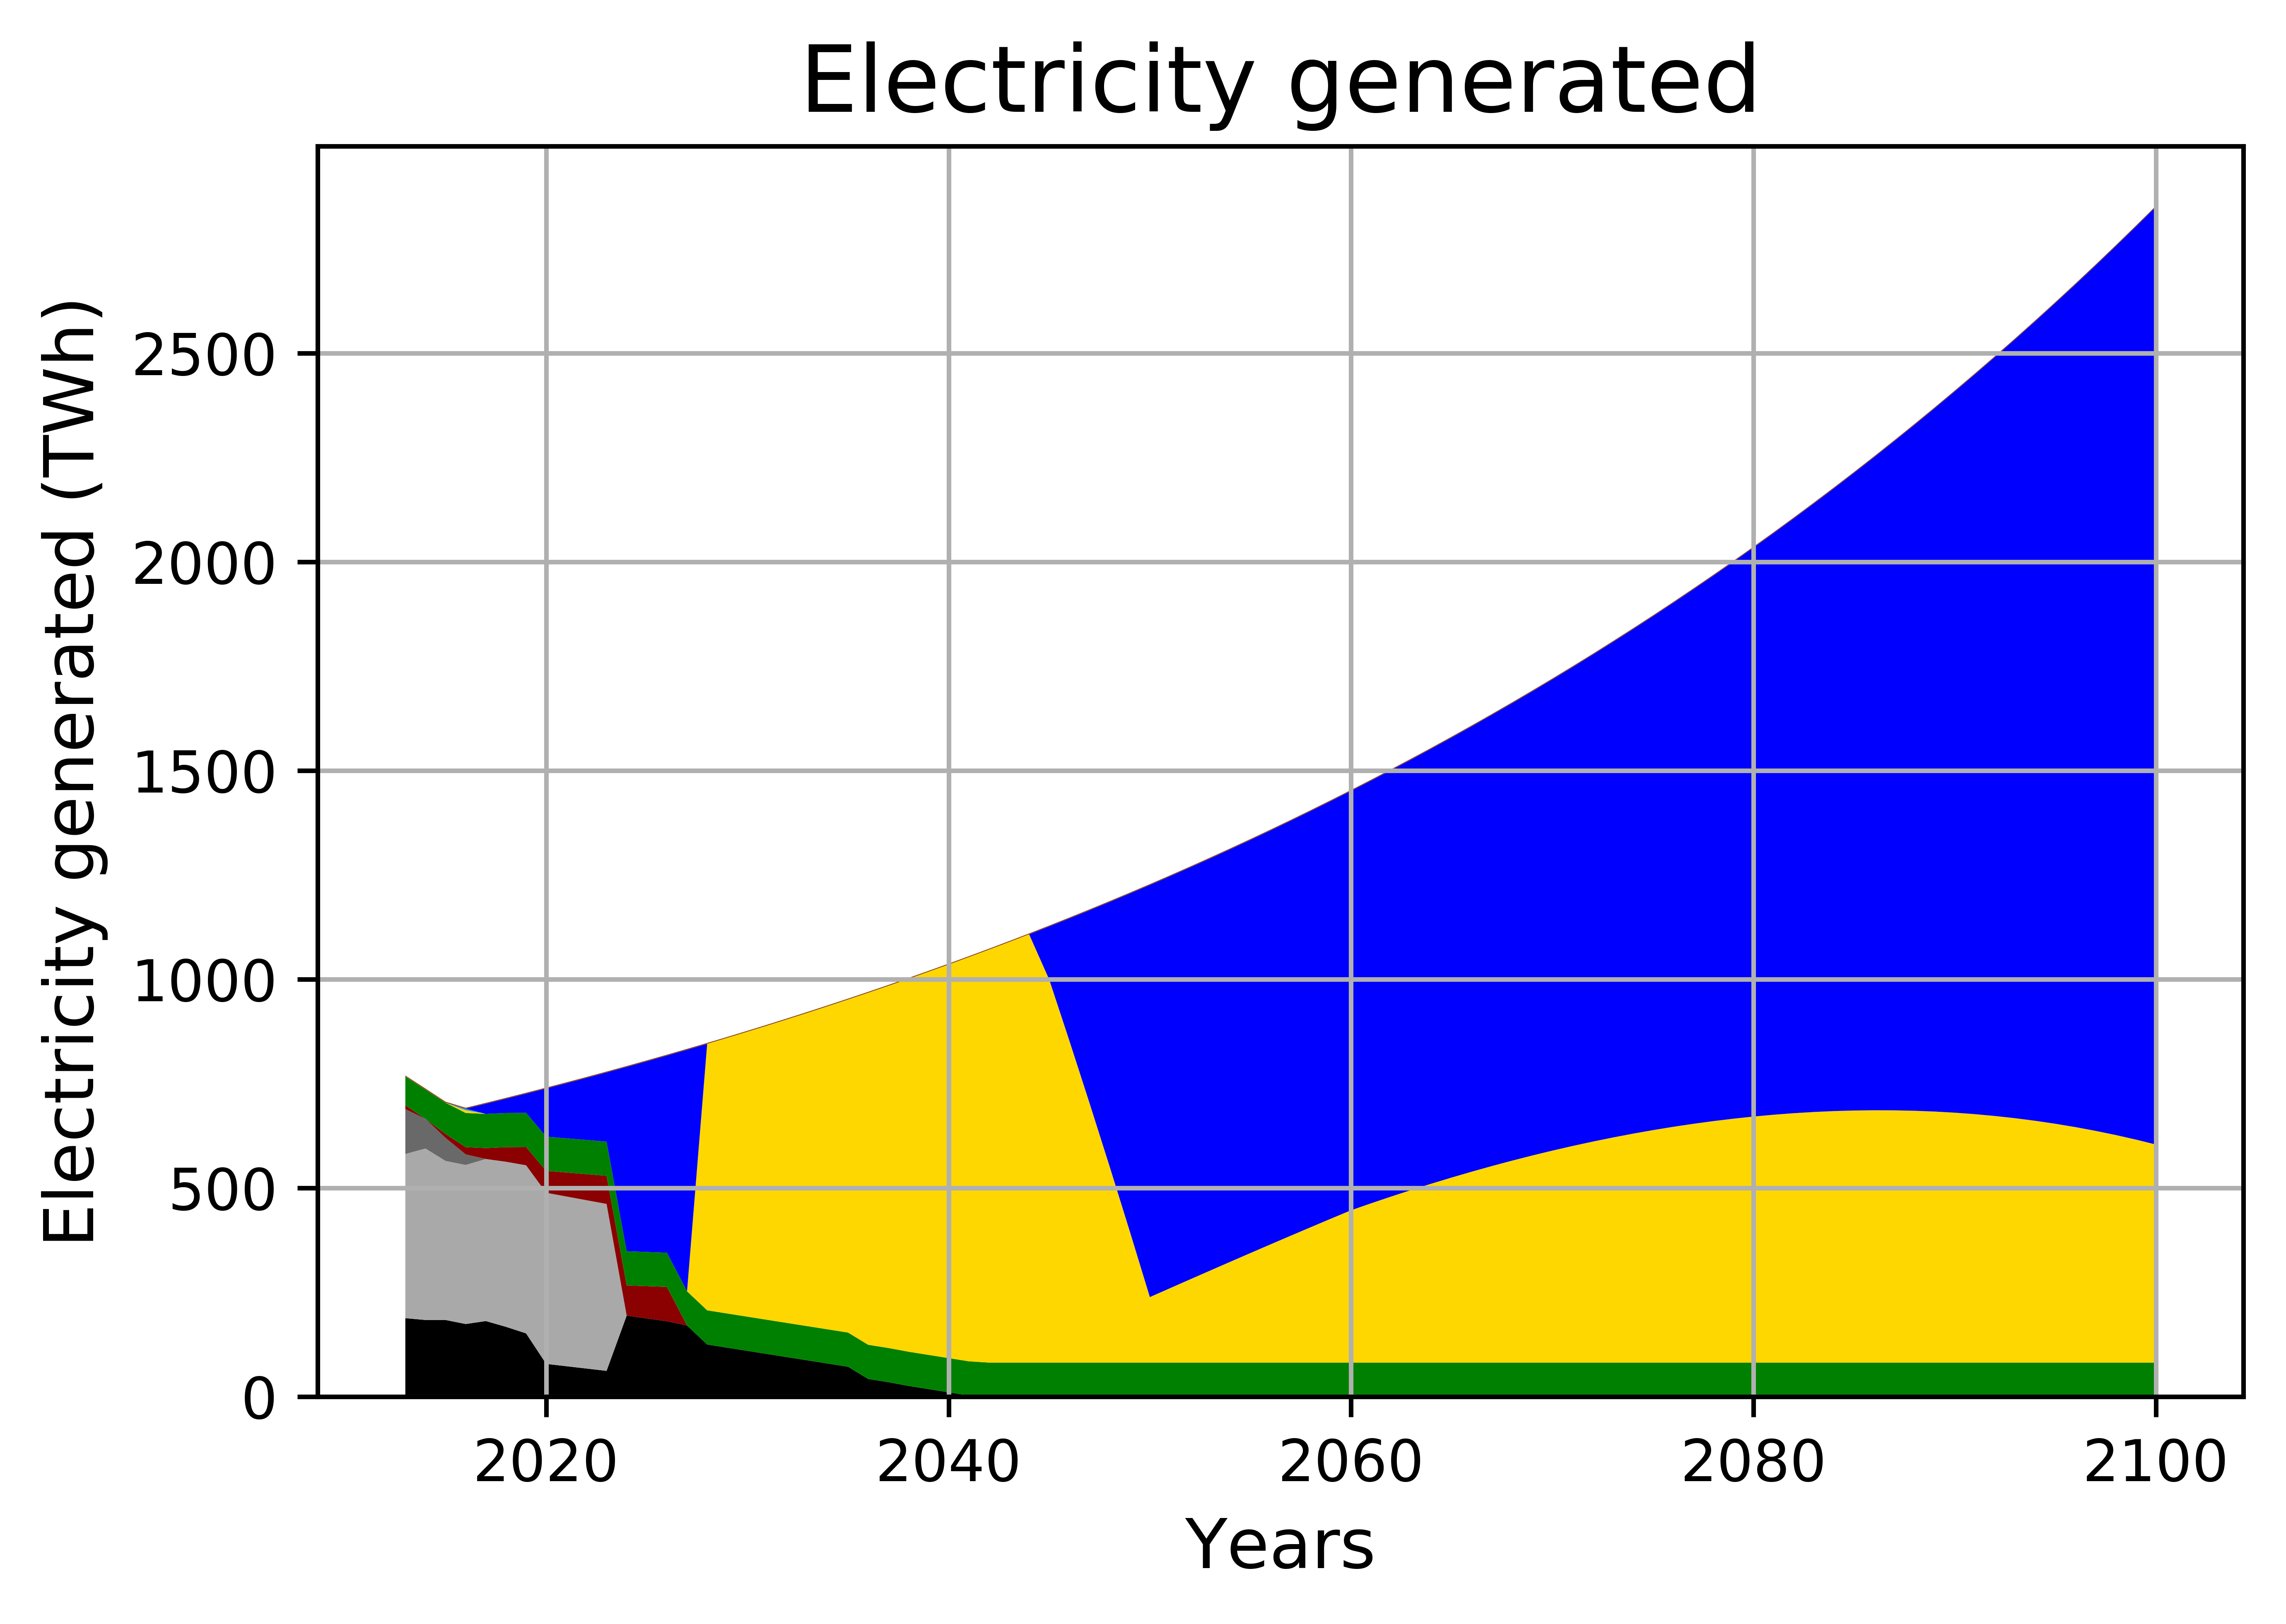
\includegraphics[scale=1.51]{conv_nonuc_elc}
\caption{\textbf{Scenario 2} (conventional, no new nuclear) Electricity Generation.}
\label{s2e}
\end{figure}

\begin{figure}[H] 
\centering
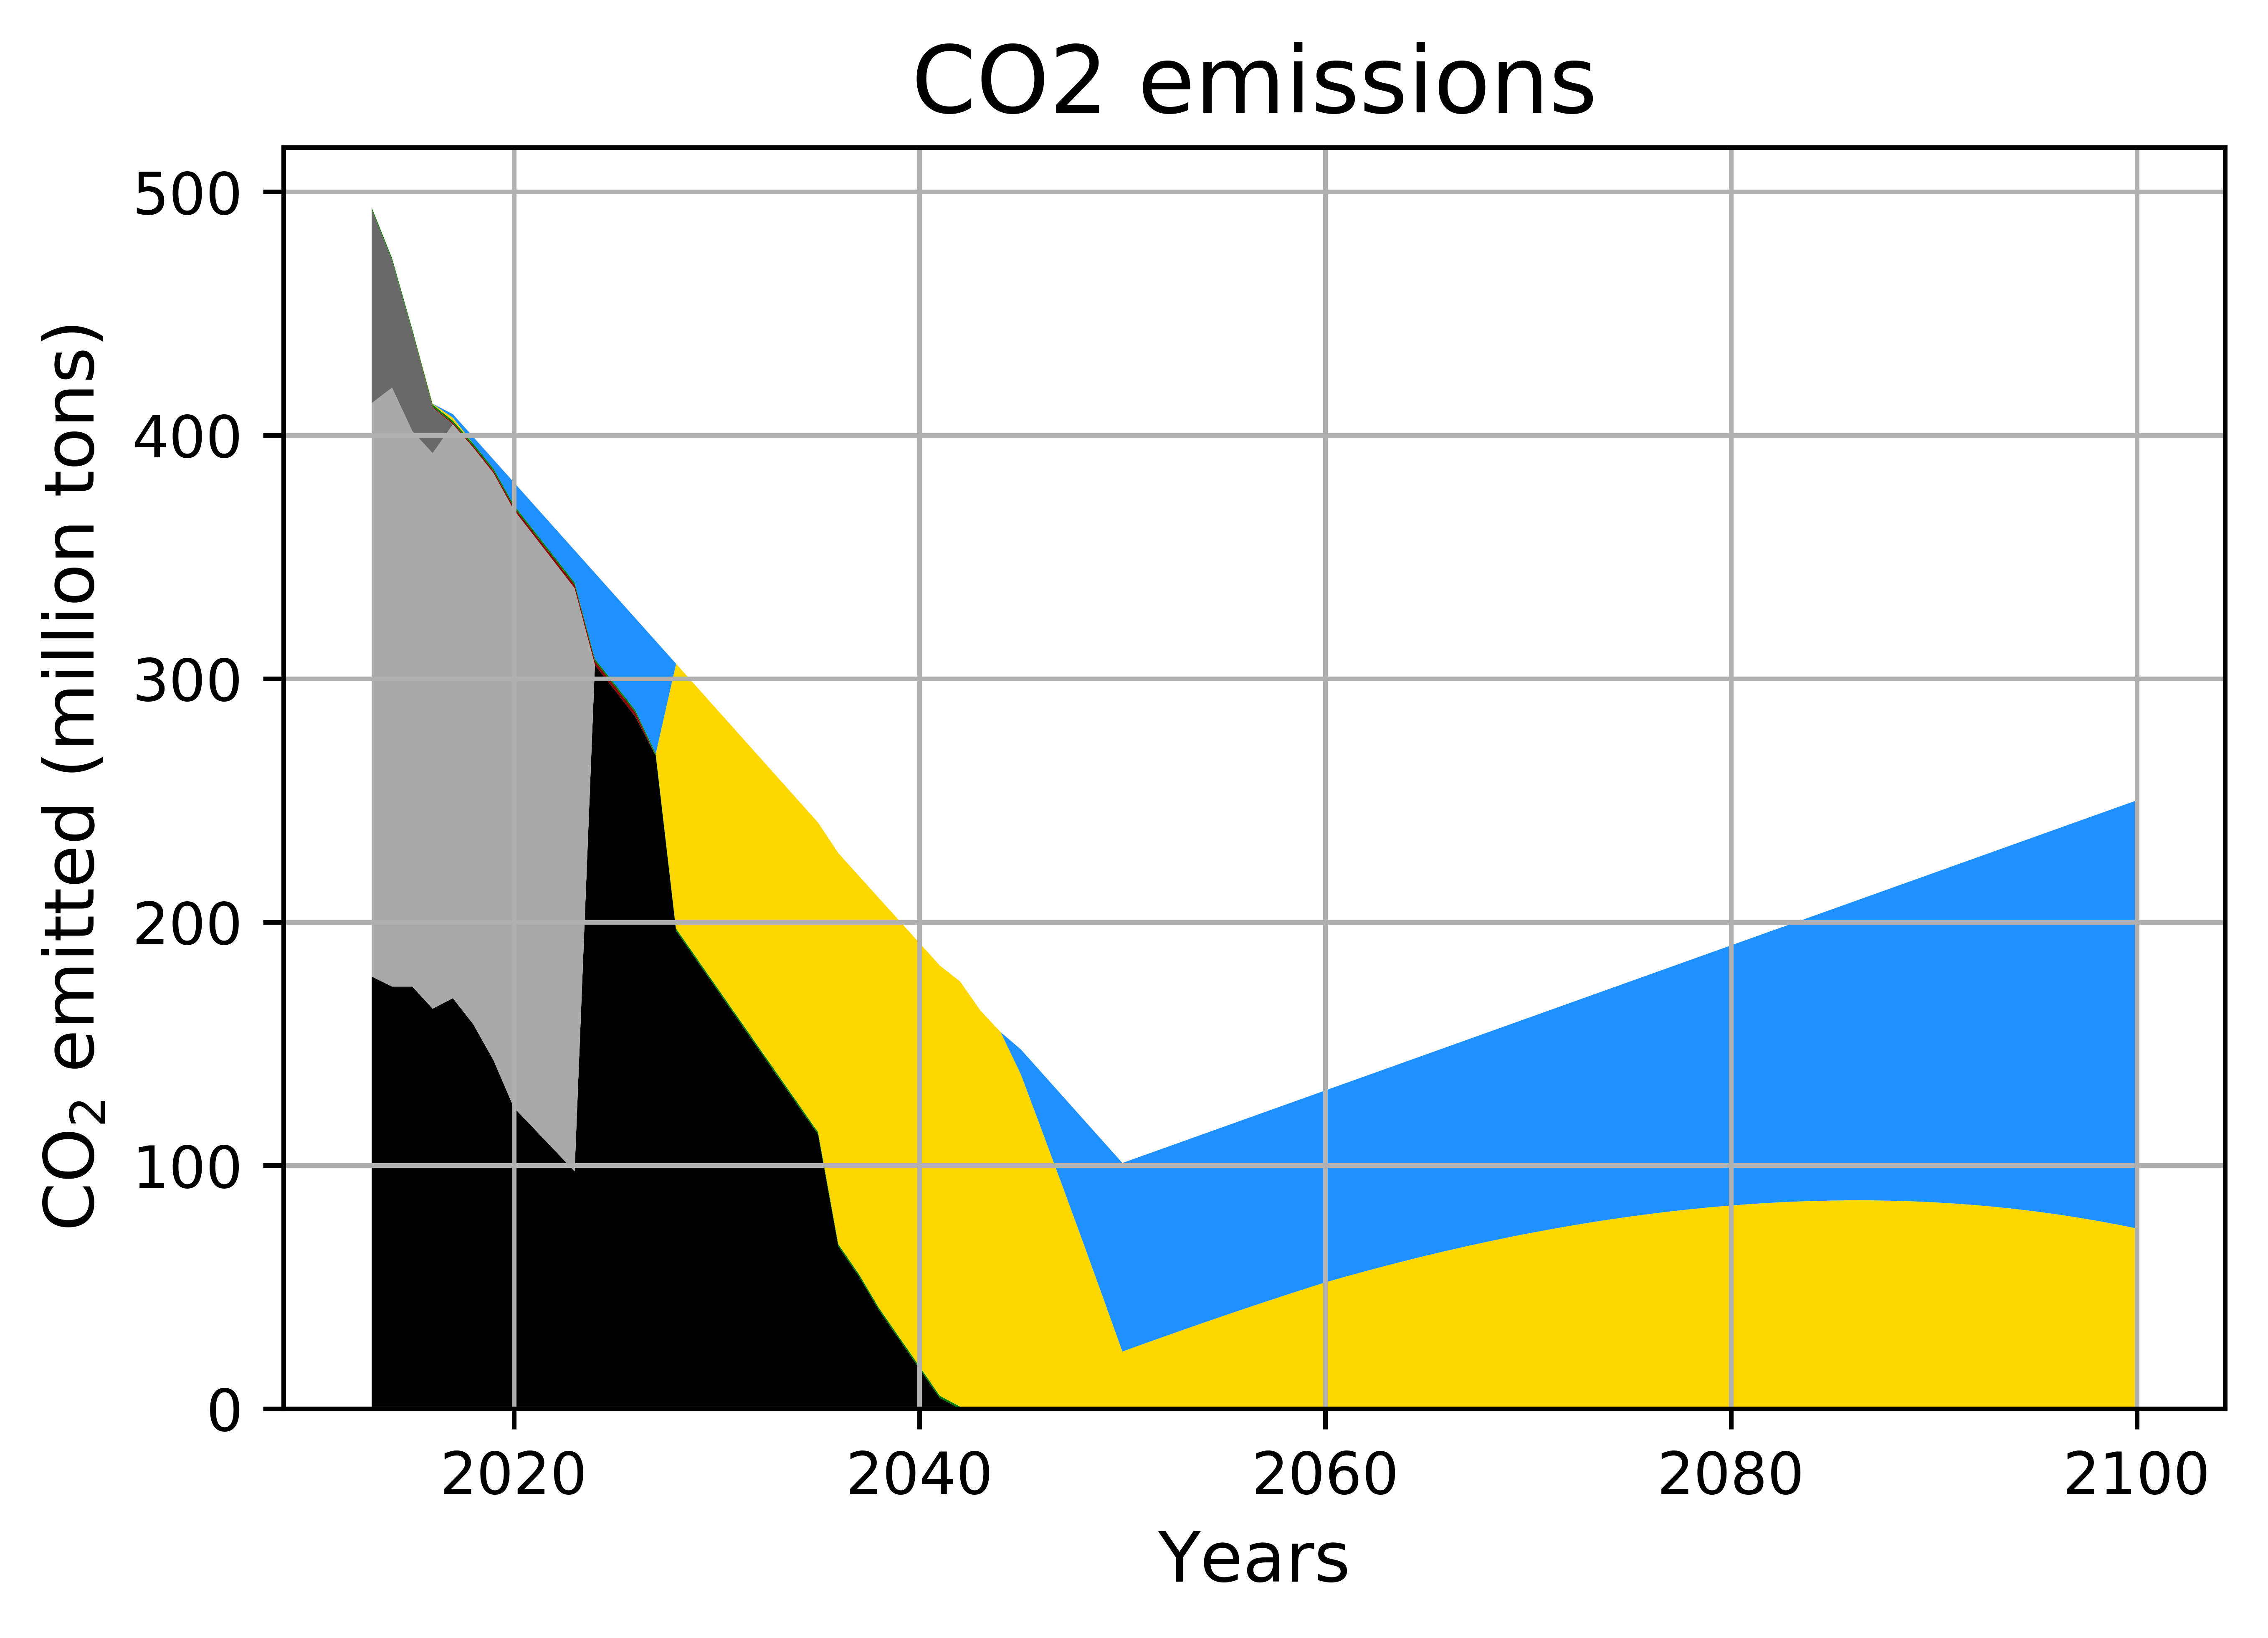
\includegraphics[scale=1.51]{conv_nonuc_co2}
\caption{\textbf{Scenario 2} (conventional, no new nuclear) CO$_2$ emissions.}
\label{s2c}
\end{figure}

%----------------------------------------------------------------------------------------

\end{column} % End of the first column

%===========================================================================================
% SECOND COLUMN BEGINS
%=============================================================================================

%----------------------------------------------------------------------------------------
\begin{column}{\onecolwid} % The second column
%----------------------------------------------------------------------------------------
\begin{block}{Methodology}
        \textbf{The Integrated MARKAL-EFOM System (TIMES)} 
        \cite{loulou_documentation_2005} 
        \cite{seebregts_energy/environmental_2002} optimizes energy systems 
        using linear \& mixed-linear algorithms. An objective 
        function is solved within given constraints.\\
\textbf{Key assumptions:}
\begin{itemize}
        \item\textbf{Objective function:} System cost (Fig. \ref{cost}). 
        
         \item\textbf{Constraints:} CO$_2$ emissions, demand(+1.7\% per year) \cite{noauthor_electricity_2017}.
         
         \item Hydropower and geothermal capacity are constant \cite{noauthor_energy_2018}.
                  
         \item All new nuclear reactors are ABWRs \cite{rothwell_real_2006}.
         
         \item Nuclear, wind, solar growth rate based on trends in USA, China, and Japan.\cite{noauthor_electricity_2017,noauthor_energy_2018,eia_international_nodate,eia_monthly_2018,iea-pvps_snapshot_2018}
         
         \item \textbf{CCS:} Deploys in 2030,costs reduce by 2050. \cite{kato_energy_2016}
         
         \item \textbf{H$_2$:} Steam reforming deploys in 2030. Photocatalytic H$_2$ deploys in 2050, assumed cost-competitive. \cite{kato_energy_2016} \cite{acar_comparative_2014} \\         
 \end{itemize}   
 
We have modeled \textbf{four scenarios}:\hfill \break

\begin{tabular}{| c | c | c | c | c |}
\hline
\textbf{Scenario}& \textbf{Figures}&\textbf{Conventional}&\textbf{I$^2$CNER}&\textbf{New nuclear}\\
                 &             &\textbf{technology}&\textbf{technology}&\textbf{reactors}\\
                  \hline
1               & Fig. \ref{s1e}\&\ref{s1c}&      \greencheck           &         \xmark       &      \greencheck     \\ 
2               & Fig. \ref{s2e}\&\ref{s2c}&      \greencheck           &         \xmark       &         \xmark       \\ 
3               & Fig. \ref{s3e}\&\ref{s3c}&      \greencheck           &      \greencheck     &      \greencheck     \\ 
4               & Fig. \ref{s4e}\&\ref{s4c}&      \greencheck           &      \greencheck     &         \xmark       \\
\hline
\end{tabular}
\end{block}

%\vspace{65 mm}

\begin{figure}[H] 
\centering
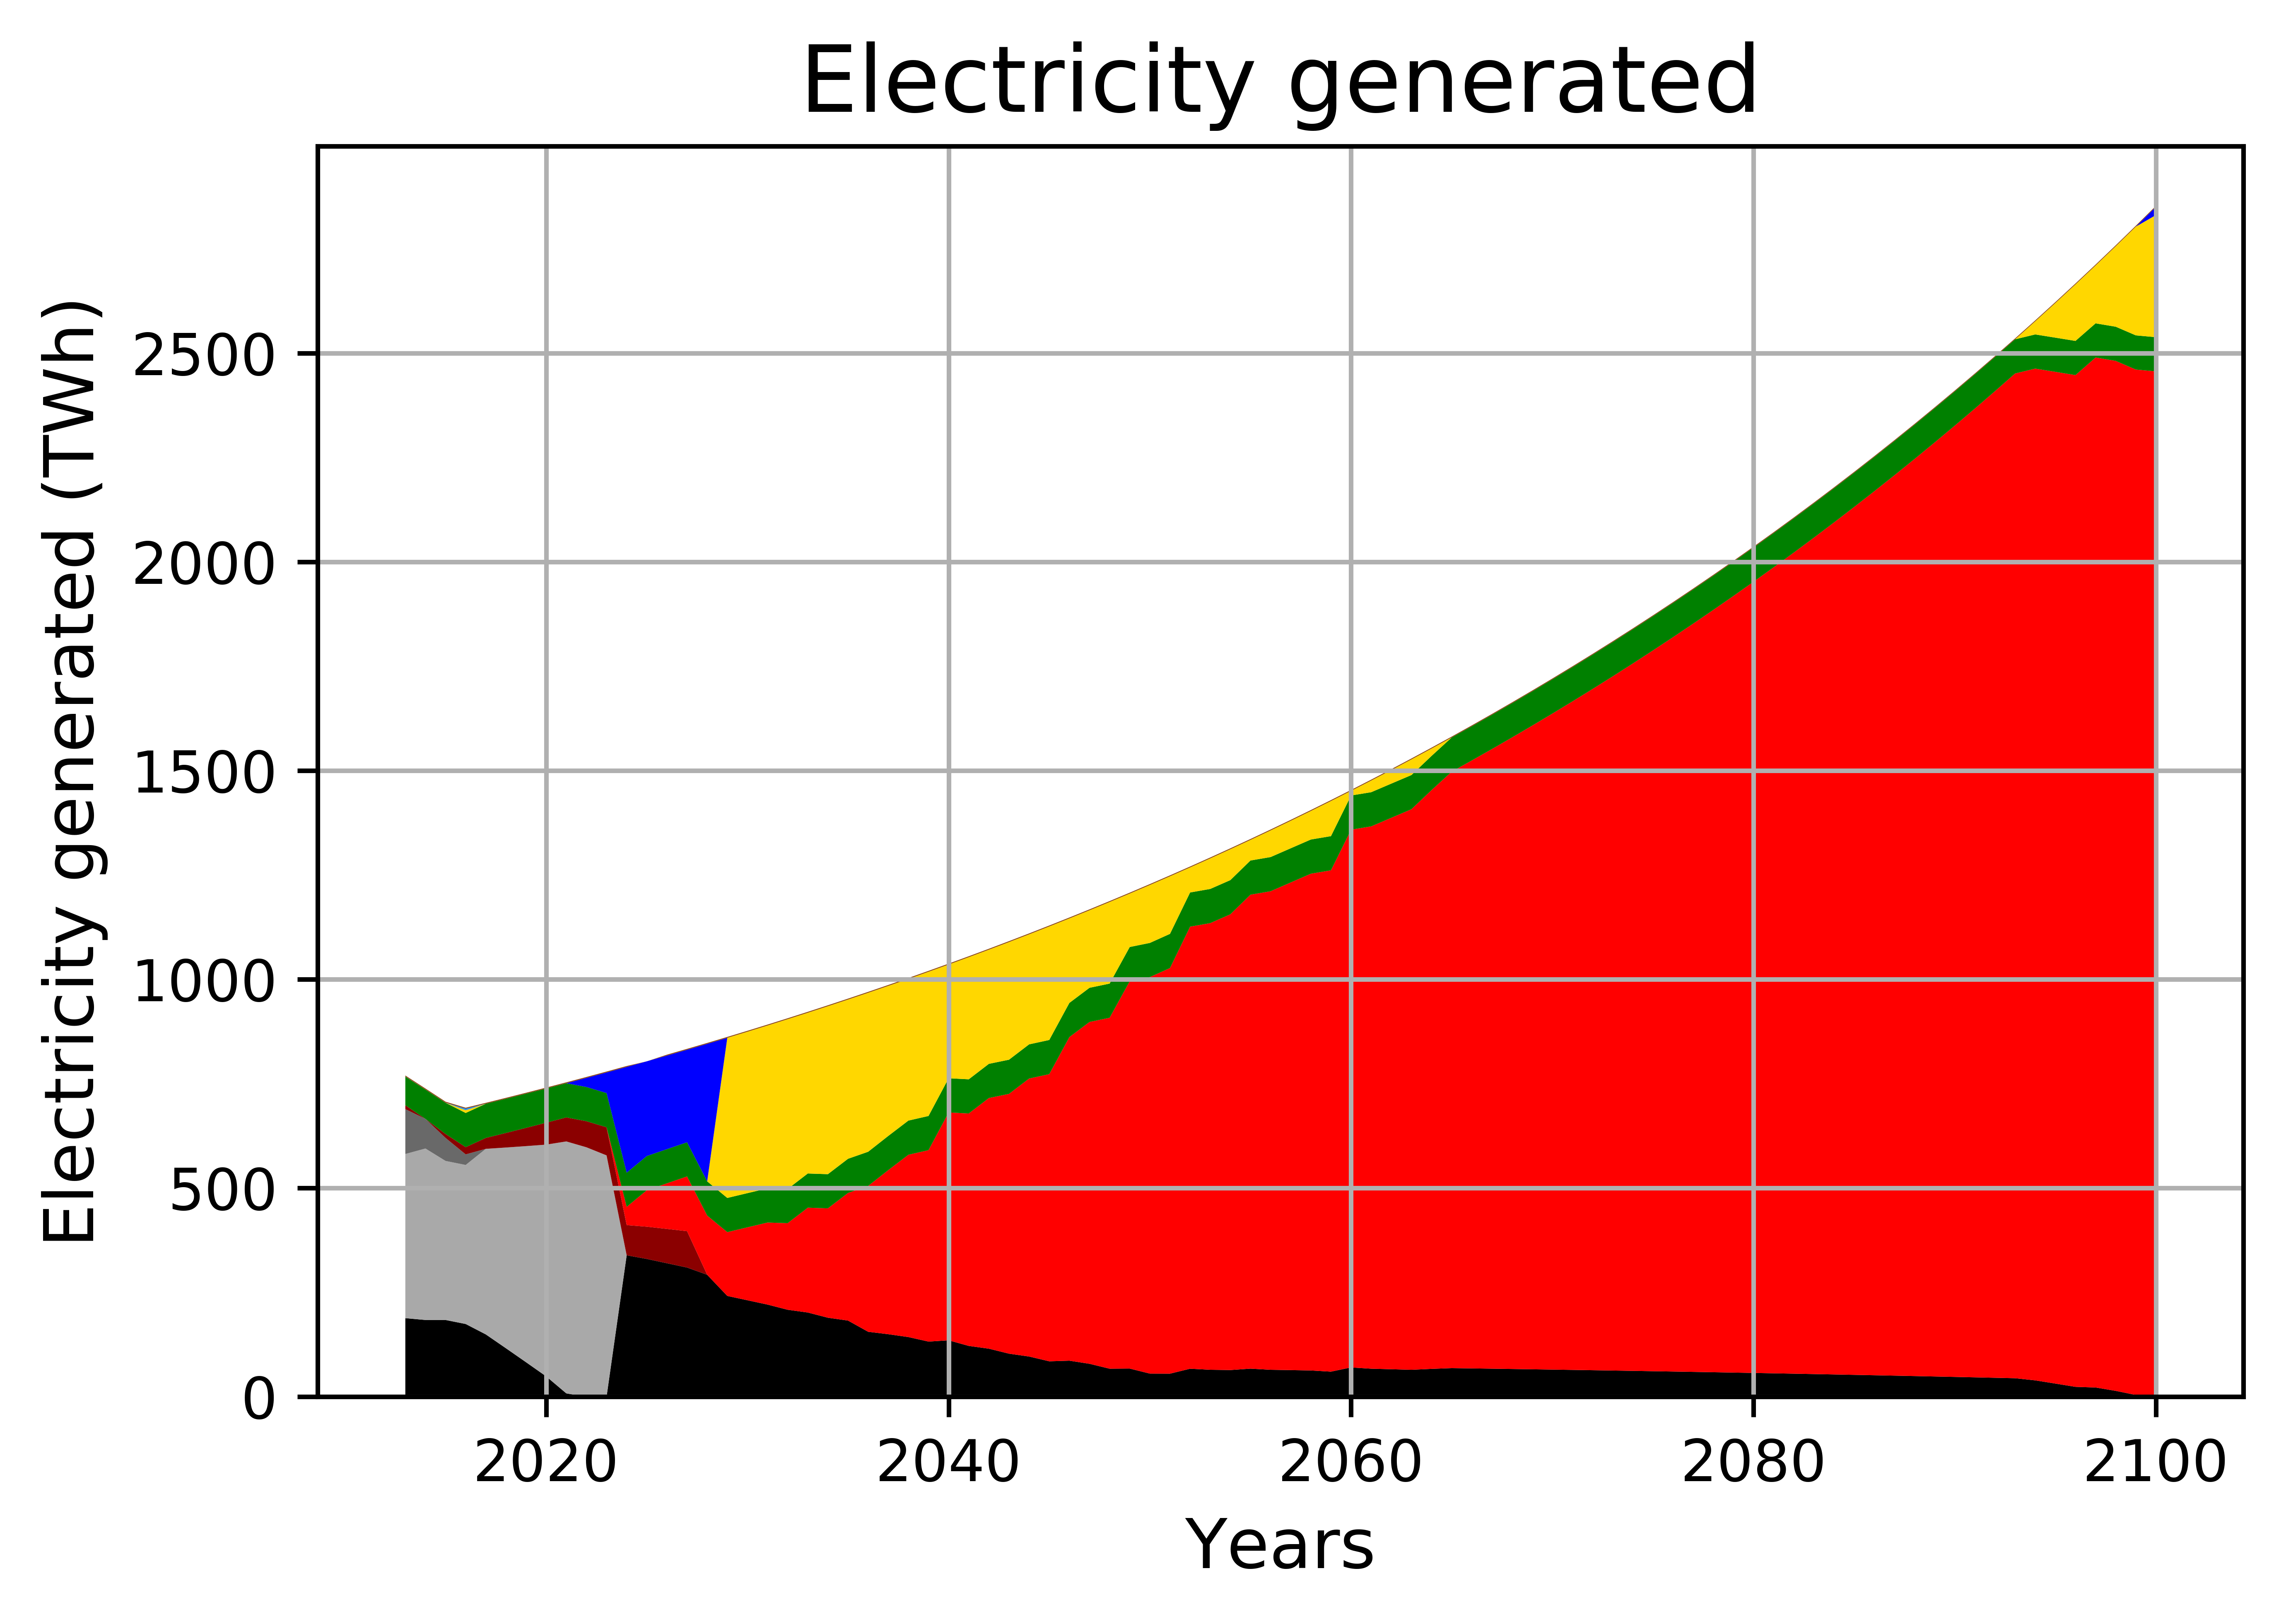
\includegraphics[scale=1.62]{i2cner_nuc_elc}
\caption{\textbf{Scenario 3} (with I$^2$CNER tech and new nuclear) Electricity Generation.}
\label{s3e}
\end{figure}

\begin{figure}[H] 
\centering
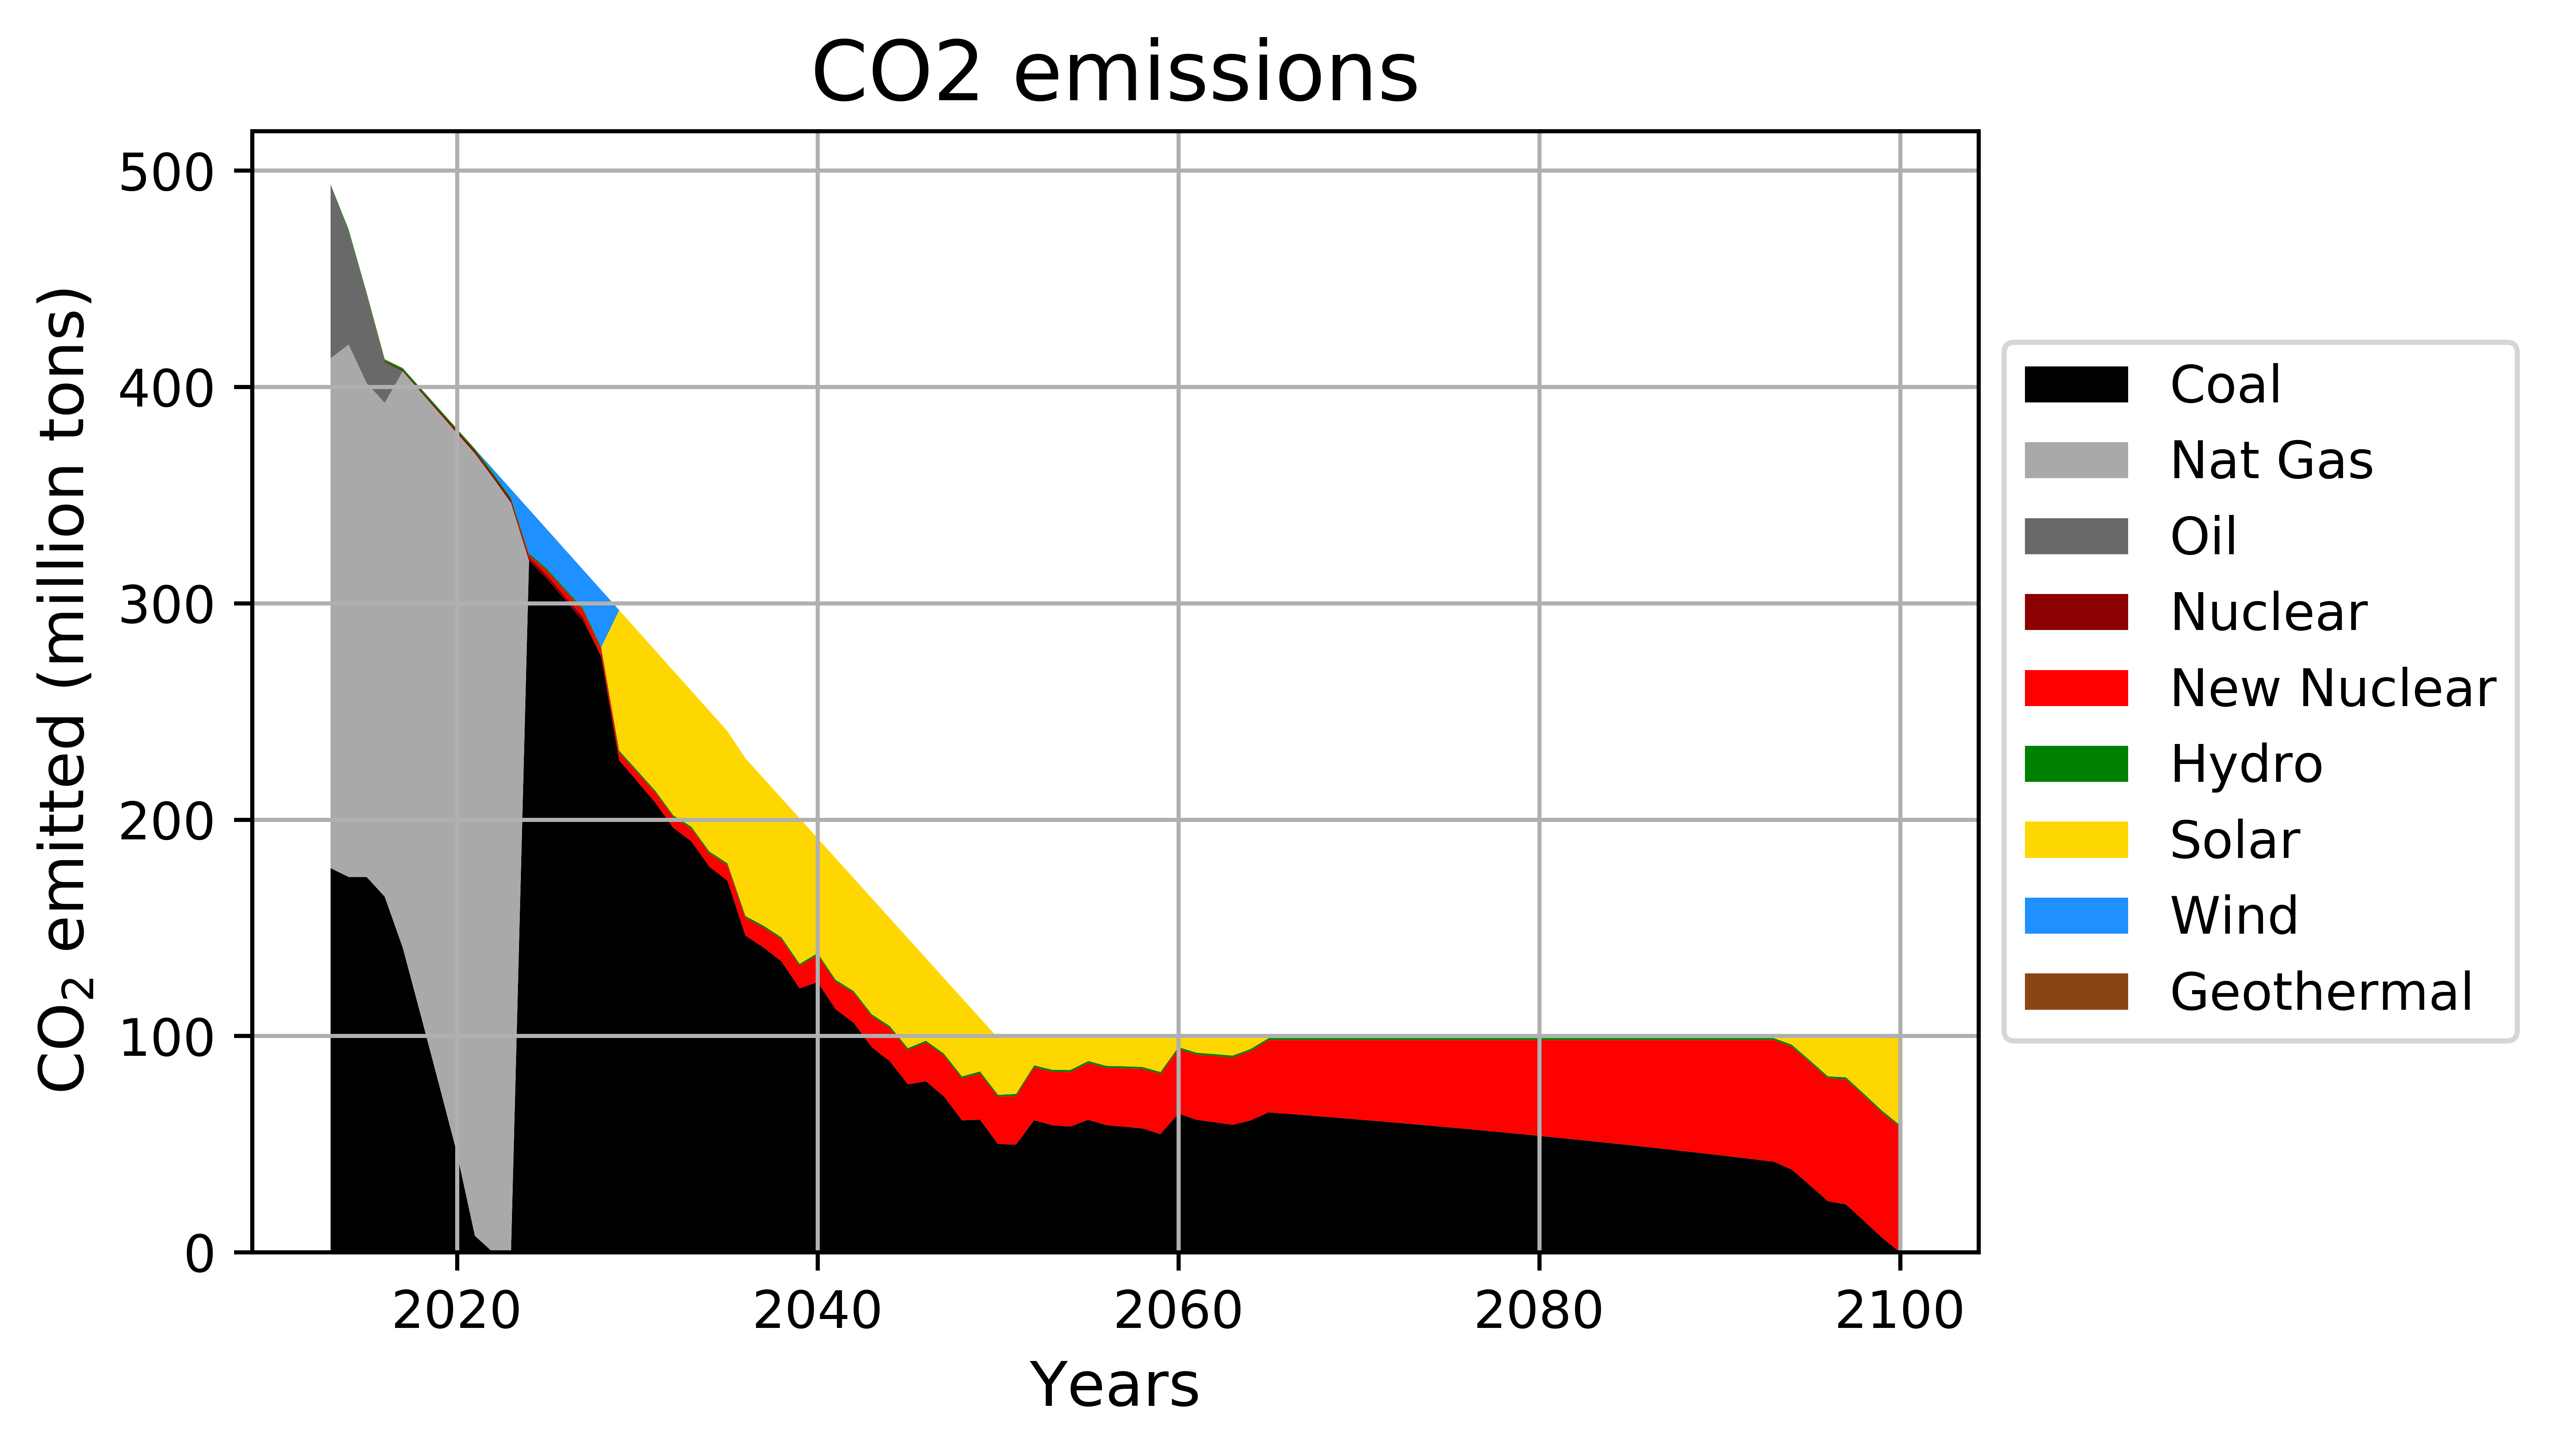
\includegraphics[scale=1.62]{i2cner_nuc_co2}
\caption{\textbf{Scenario 3} (with I$^2$CNER tech and new nuclear) CO$_2$ emissions.}
\label{s3c}
\end{figure}


\begin{figure}[H] 
\centering
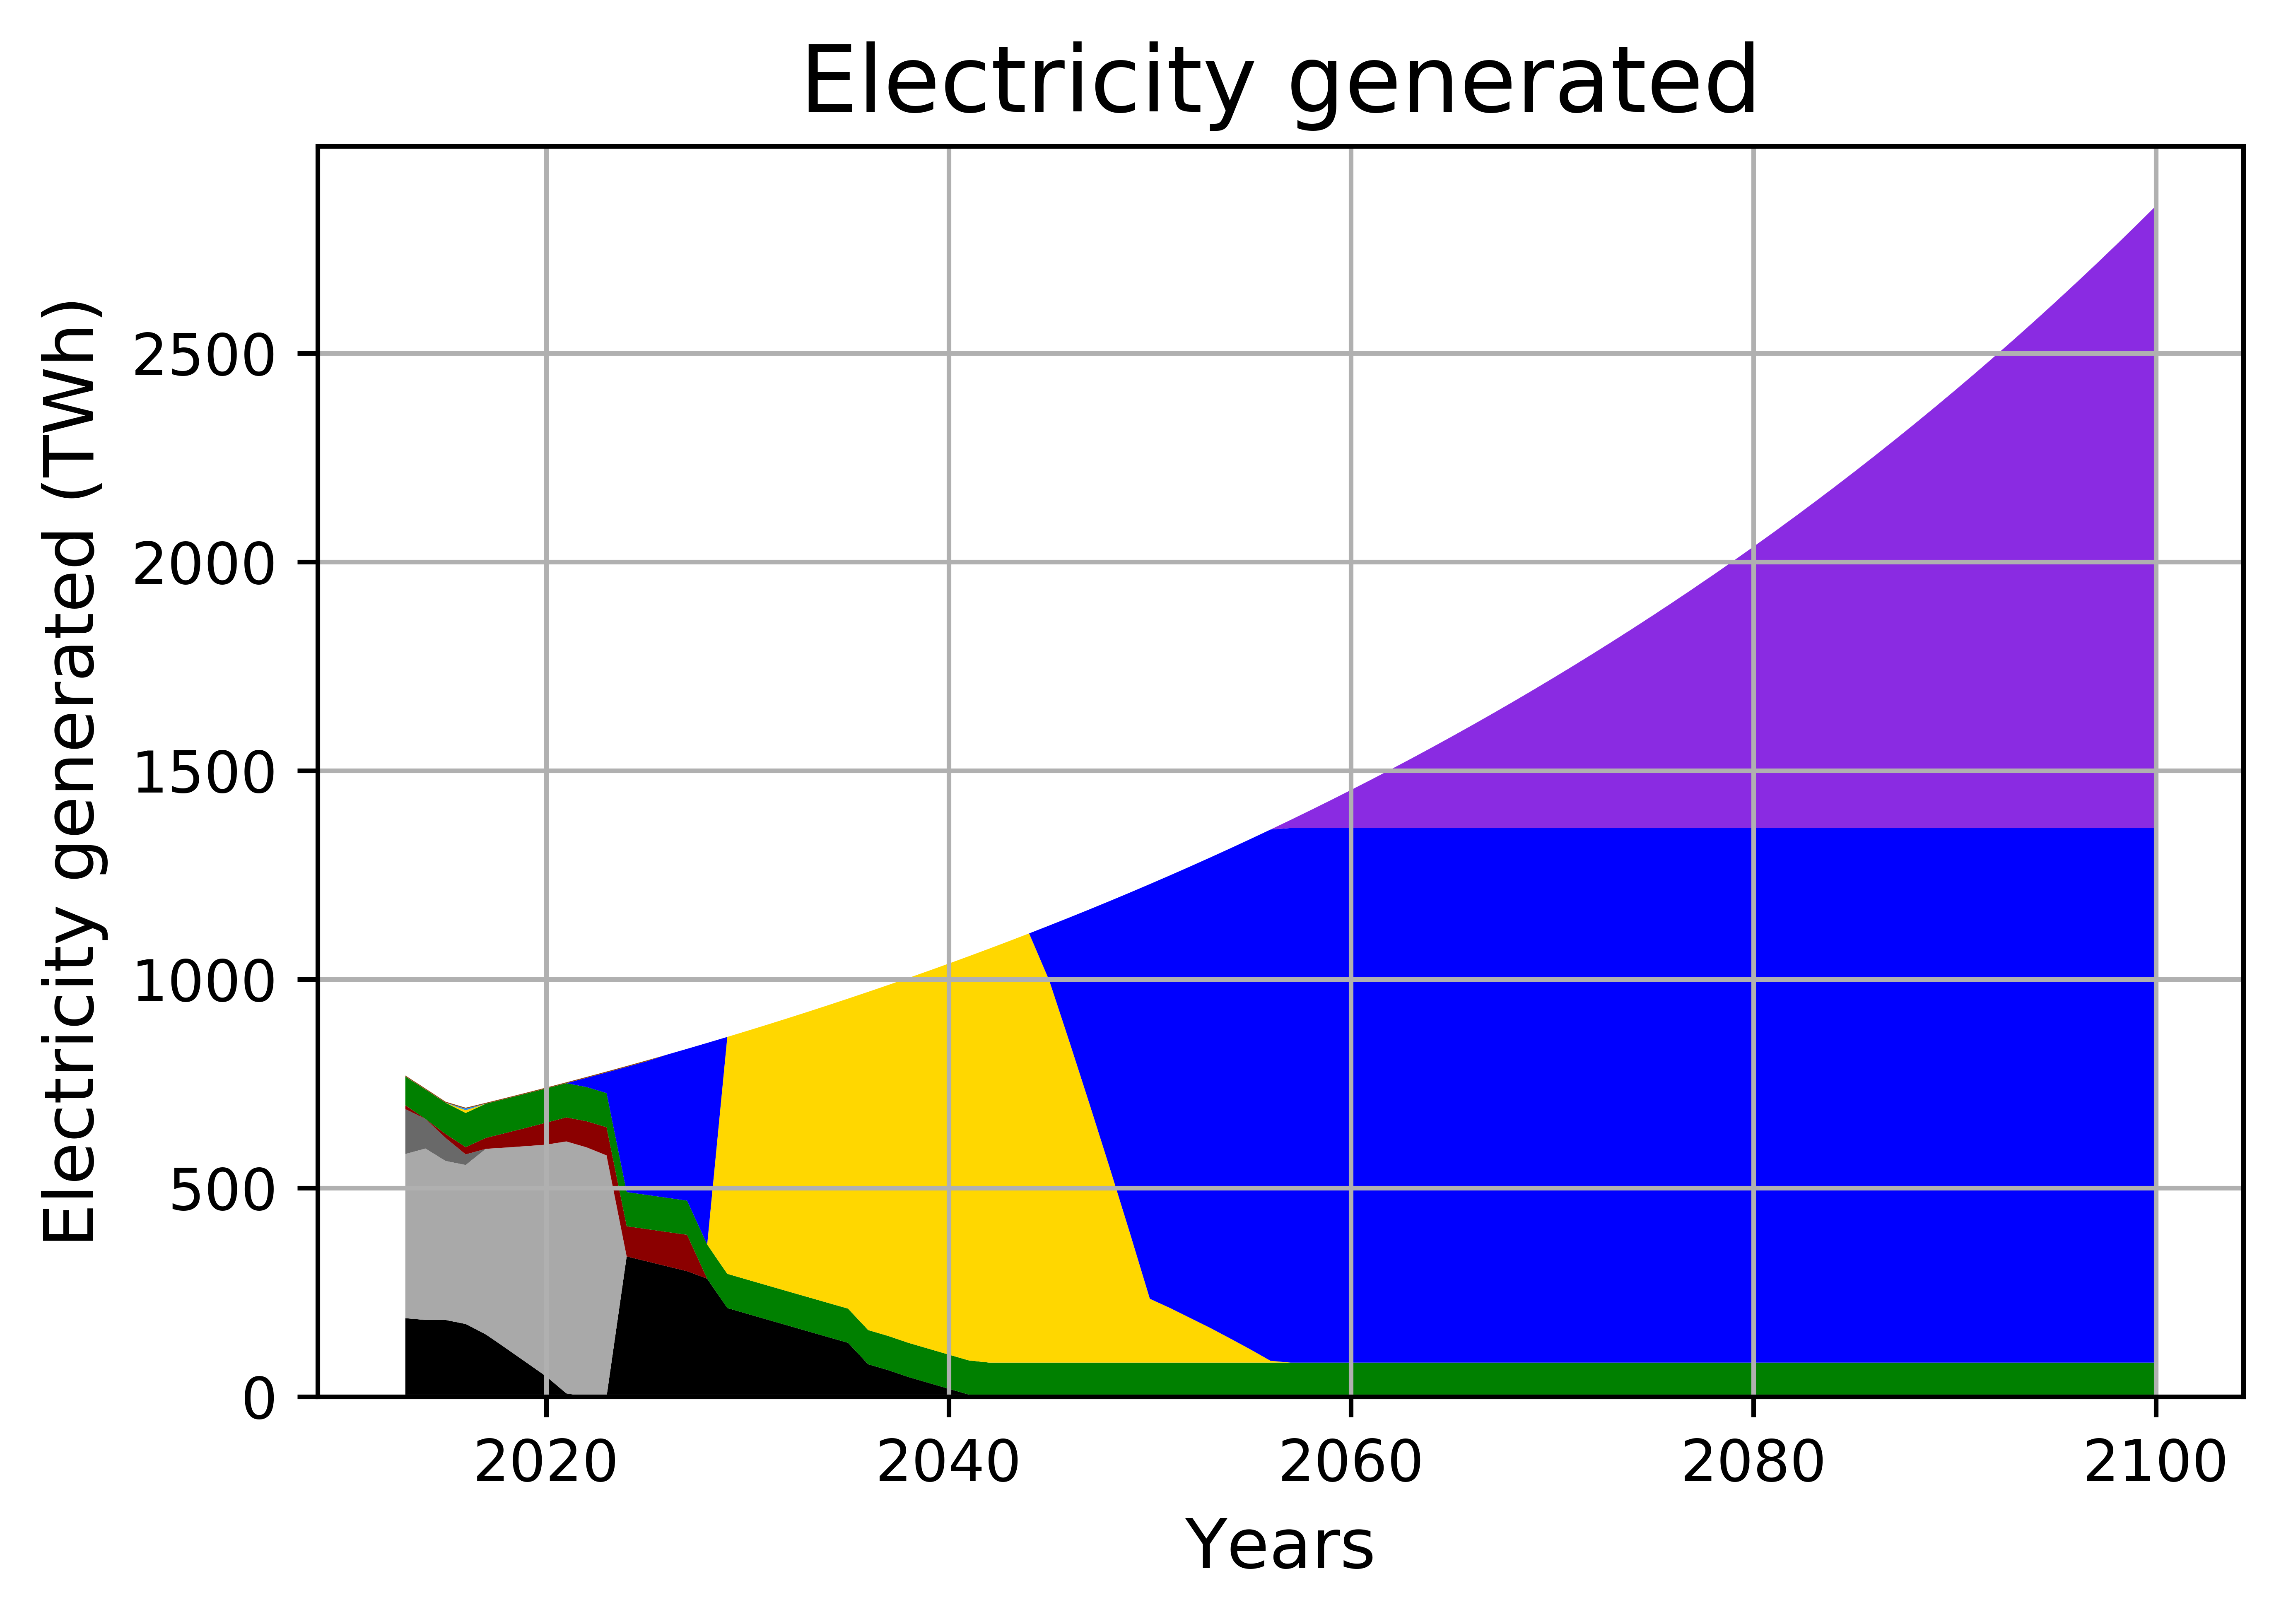
\includegraphics[scale=1.62]{i2cner_nonuc_elc}
\caption{\textbf{Scenario 4} (with I$^2$CNER tech, no new nuclear) Electricity Generation.}
\label{s4e}
\end{figure}

\begin{figure}[H] 
\centering
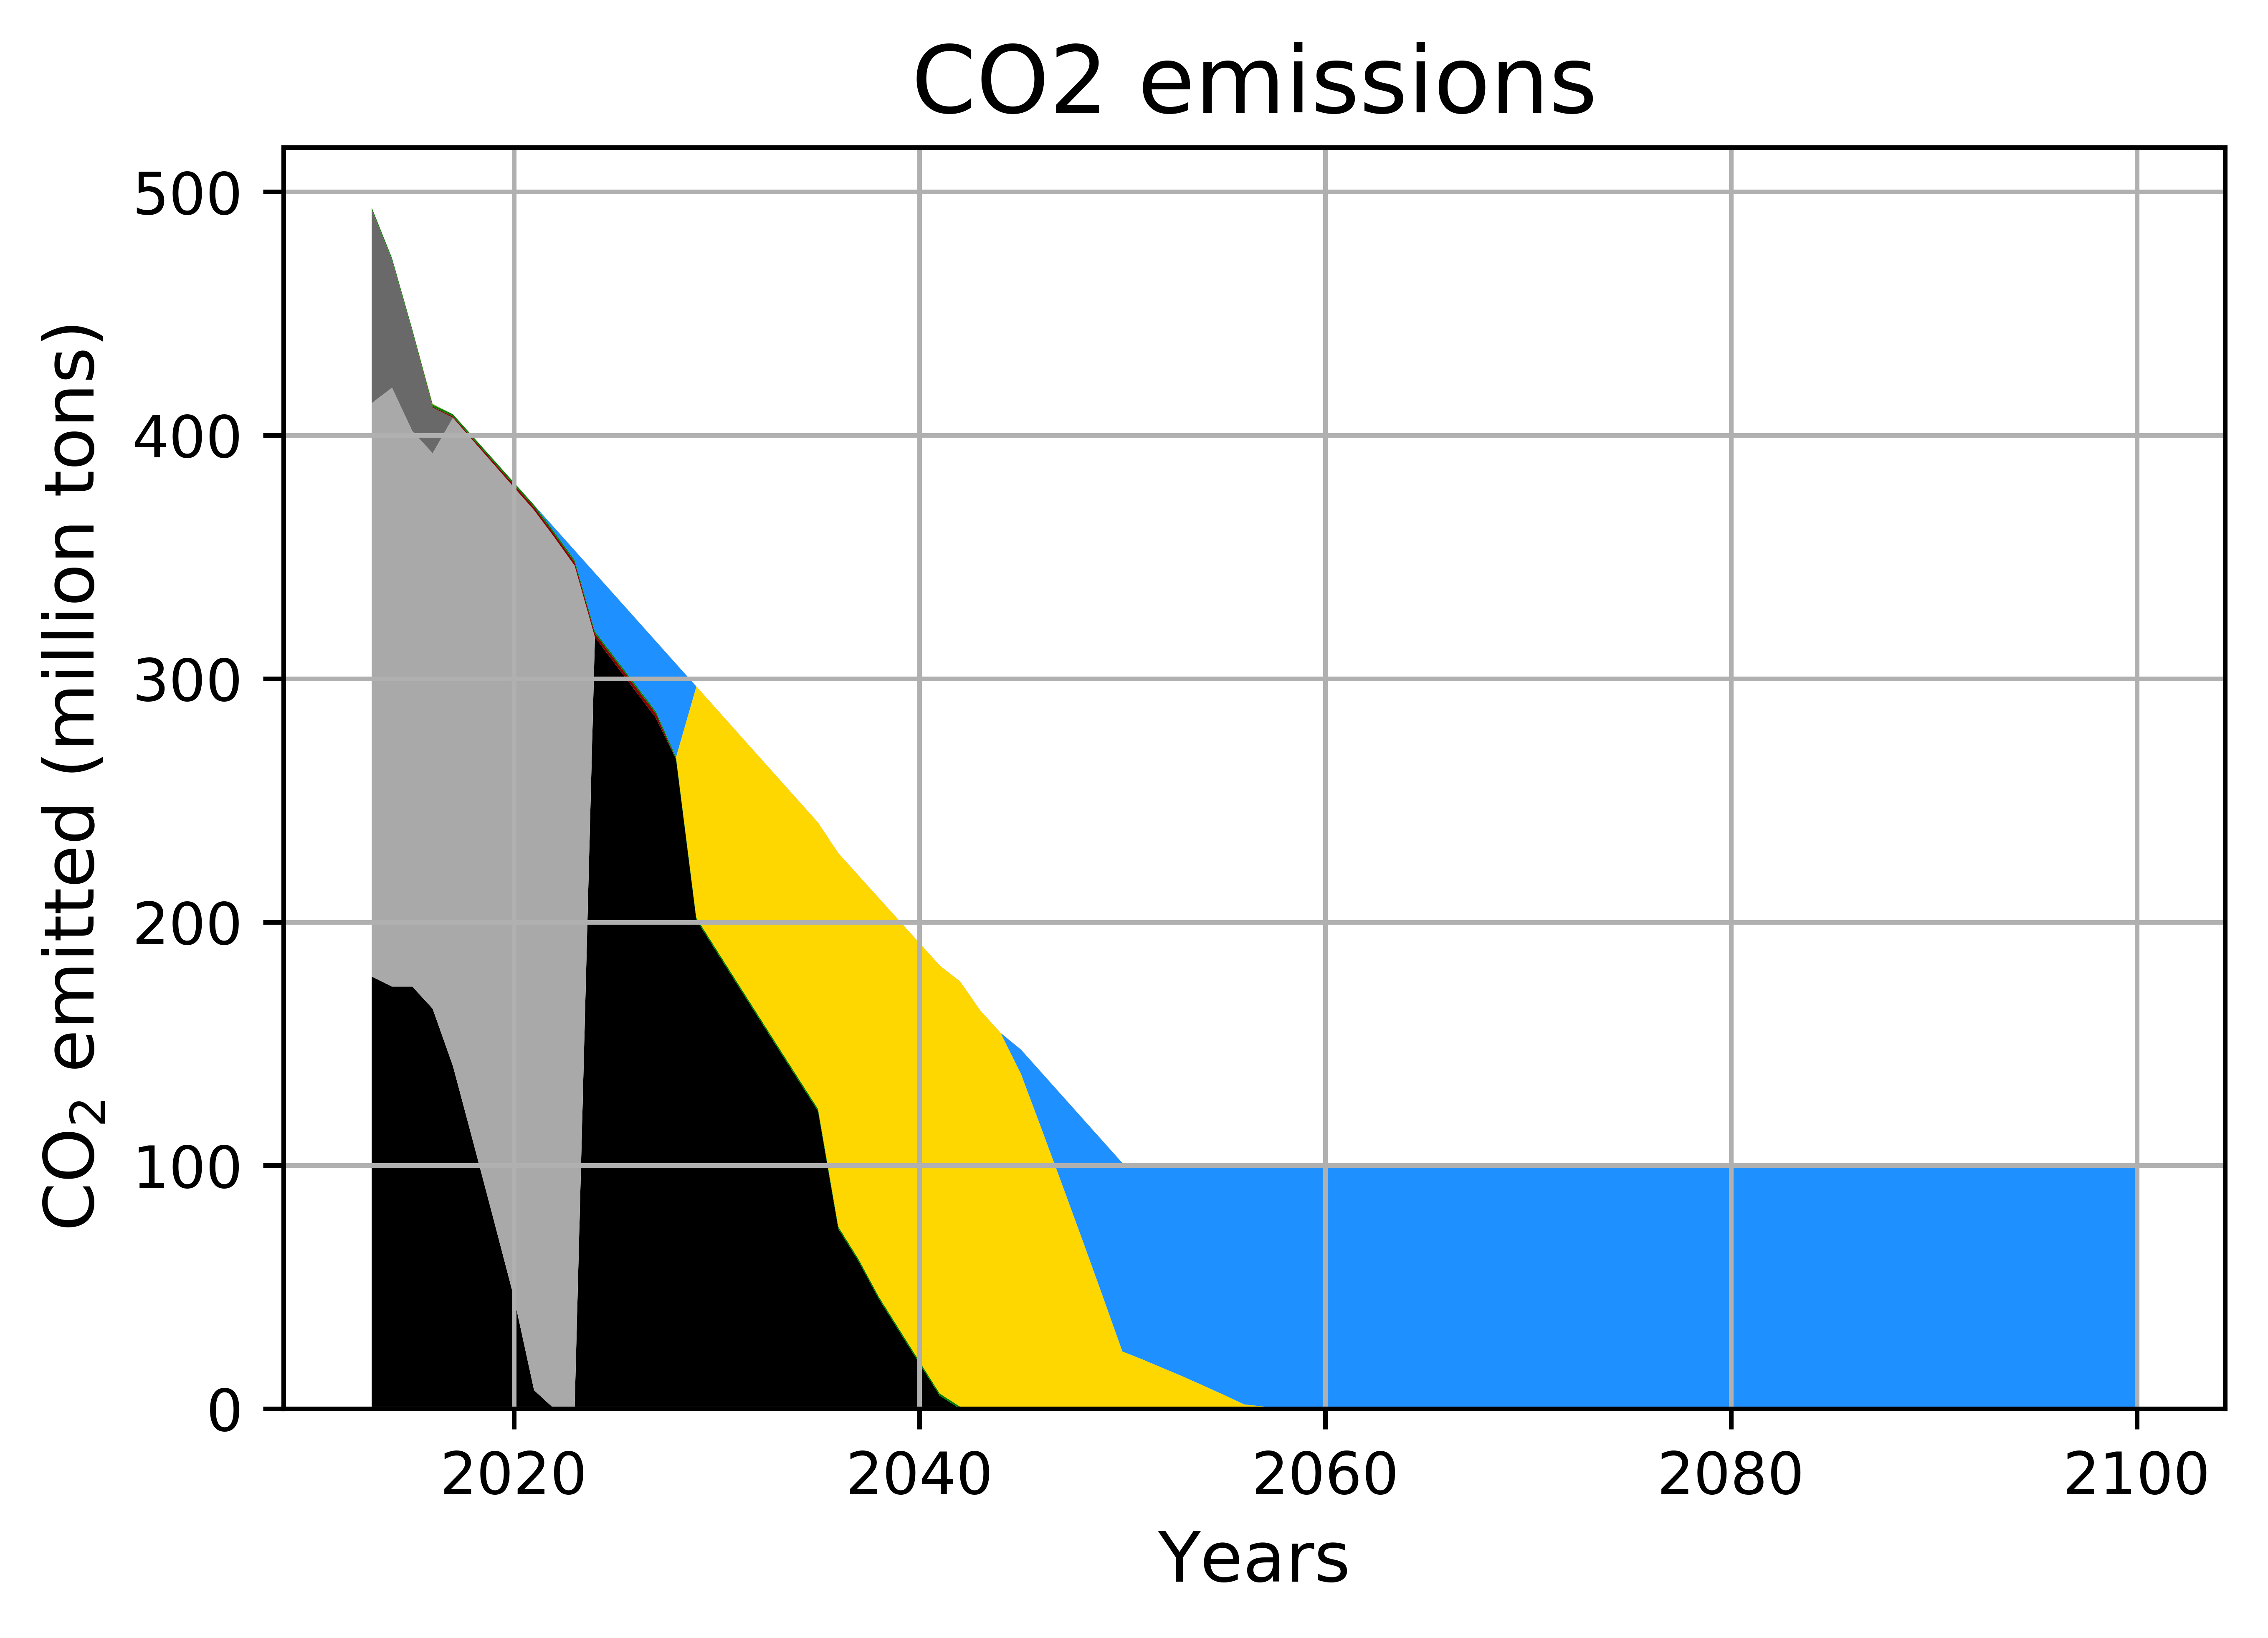
\includegraphics[scale=1.62]{i2cner_nonuc_co2}
\caption{\textbf{Scenario 4} (with I$^2$CNER tech, no new nuclear) CO$_2$ emissions.}
\label{s4c}
\end{figure}

\end{column} % End of column 2, top half
\end{columns}
%=======================================================
% Double Wide Figure Column 
%=========================================================
%
%=======================================================
% FIGURE BEGINS
%=========================================================

% tell TikZ how to stack them (back to front)
\newlength{\figwidth}
\setlength{\figwidth}{8cm}

\begin{figure}
    \centering
    \scalebox{1.0}{
                \begin{tikzpicture}[>={Latex[width=6mm,length=6mm]},
                                node distance=\figwidth,
                                on grid,
                                align=center,
                                auto]
        % Place nodes
        \node [block] (times) {\textbf{TIMES Model Generator}};
        \node [cloud, below=\figwidth of times] (mod) {\texttt{MODEL} \\ heterogeneous \\ multi-technology \\ model of Japan};
                \node [cloud, above left=1.5\figwidth and 2*\figwidth of times]
                (dat) {\texttt{DATA}\\regarding both\\i$^2$cner and\\ conventional\\technologies};
                \node [data, above=1.5\figwidth of dat] (dat1) {Storage\\Capacity};
                \node [data, above=0.5\figwidth of dat1] (dat2) {Thermal\\Efficiency};
                \node [data, above=0.5\figwidth of dat2] (dat3) {Capacity\\factor};
                \node [data, above=0.5\figwidth of dat3] (dat4) {Availability\\factor};
                \node [data, right=\figwidth of dat1] (dat5) {Thermal\\capacity};
                \node [data, above=0.5\figwidth of dat5] (dat6) {Fuel costs};
                \node [data, above=0.5\figwidth of dat6] (dat7) {Construction\\costs};
                \node [data, above=0.5\figwidth of dat7] (dat8) {Operation\\costs};
                \node [data, above=0.5\figwidth of dat8] (dat9) {Maintenance\\costs};
                \node [data, right=\figwidth of dat5] (dat10) {Technology\\readiness};
                \node [data, above=0.5\figwidth of dat10] (dat11) {Construction\\time};
                \node [data, above=0.5\figwidth of dat11] (dat12) {Carbon\\intensity};
                \node [data, above=0.5\figwidth of dat12] (dat13) {Fuel needs};
        \node [cloud, above=\figwidth of times] (of) {\texttt{OBJECTIVE}\\\texttt{FUNCTION}};
        \node [block, above left=\figwidth of of] (min) {Minimize\\carbon emissions \\ from all sources};
        \node [block, above right=\figwidth of of] (max) {Maximize\\energy market\\ diversity};
        \node [cloud, above right=1.5*\figwidth and 2*\figwidth of times] (const) {\texttt{CONSTRAINTS} \\ e.g.: Deployed \\ sources must\\ meet energy \\ demand};
        \node [const, above=\figwidth of const ] (dem) {electricity\\demand growth};
        \node [const, left=\figwidth of dem ] (init) {initial\\condition (2010)};
        \node [const, above=0.5*\figwidth of dem] (infra) {infrastructure\\availability};
        \node [const, left=\figwidth of infra] (sec) {consumption\\by sector};
        \node [const, above=0.5*\figwidth of infra] (reg) {regional\\transmission};
        
        \begin{scope}[on background layer]
        \draw[->, ultra thick] let \p1=($(times)-(dat)$) in (dat) -- +(0,\y1)-- +(times);
        \draw[->, ultra thick] (of) -- (times);
        %\draw[->, ultra thick] let \p3=($(times)-(const)+(2,3)$),\p4=($(times)+(9,9)$),\p5=($(const)-(3,3)$) in (\x3,\y4) -- +(0,\y2)-- +(times);
        \draw[->, ultra thick] let \p2=($(times)-(const)$) in (const)-- +(0,\y2) -- + (times);
                \draw[->, ultra thick] (times) -- (mod);
        \draw[->, ultra thick] (min) -- (of);
        \draw[->, ultra thick] (max) -- (of);
        \draw[->, ultra thick] (dem) -- (const);
        \draw[->, ultra thick] (dat1) -- (dat);
        \draw[->, ultra thick] (dat2) -- (dat);
        \draw[->, ultra thick] (dat3) -- (dat);
        \draw[->, ultra thick] (dat4) -- (dat);
        \draw[->, ultra thick] (dat5) -- (dat);
        \draw[->, ultra thick] (dat6) -- (dat);
        \draw[->, ultra thick] (dat7) -- (dat);
        \draw[->, ultra thick] (dat8) -- (dat);
        \draw[->, ultra thick] (dat9) -- (dat);
        \draw[->, ultra thick] (dat10) -- (dat);
        \draw[->, ultra thick] (dat11) -- (dat);
        \draw[->, ultra thick] (dat12) -- (dat);
        \draw[->, ultra thick] (dat13) -- (dat);
        \draw[->, ultra thick] (reg) -- (const);
        \draw[->, ultra thick] (infra) -- (const);
        \draw[->, ultra thick] (sec) -- (const);
        \draw[->, ultra thick] (init) -- (const);
                \path[->] (mod) edge [ultra thick,out=330,in=0,looseness=10] (mod) node[above right=0.1\figwidth and 0.8\figwidth] {simulate\\2010-2050};
                %\draw (mod.east) to [->, ultra thick,looseness=10] (mod.south) node[above right=0.1\figwidth and 0.1\figwidth] {simulate\\2010-2050};
        \end{scope}
 \end{tikzpicture}
    }
    \caption{Basic methodology for dynamic simulation of Japan's energy system.}
\end{figure}



\end{column} % End of wide column, total length

\begin{column}{\onecolwid} % The third column

%----------------------------------------------------------------------------------------
%	TAKE AWAY
%----------------------------------------------------------------------------------------
\begin{figure}[H] 
\centering
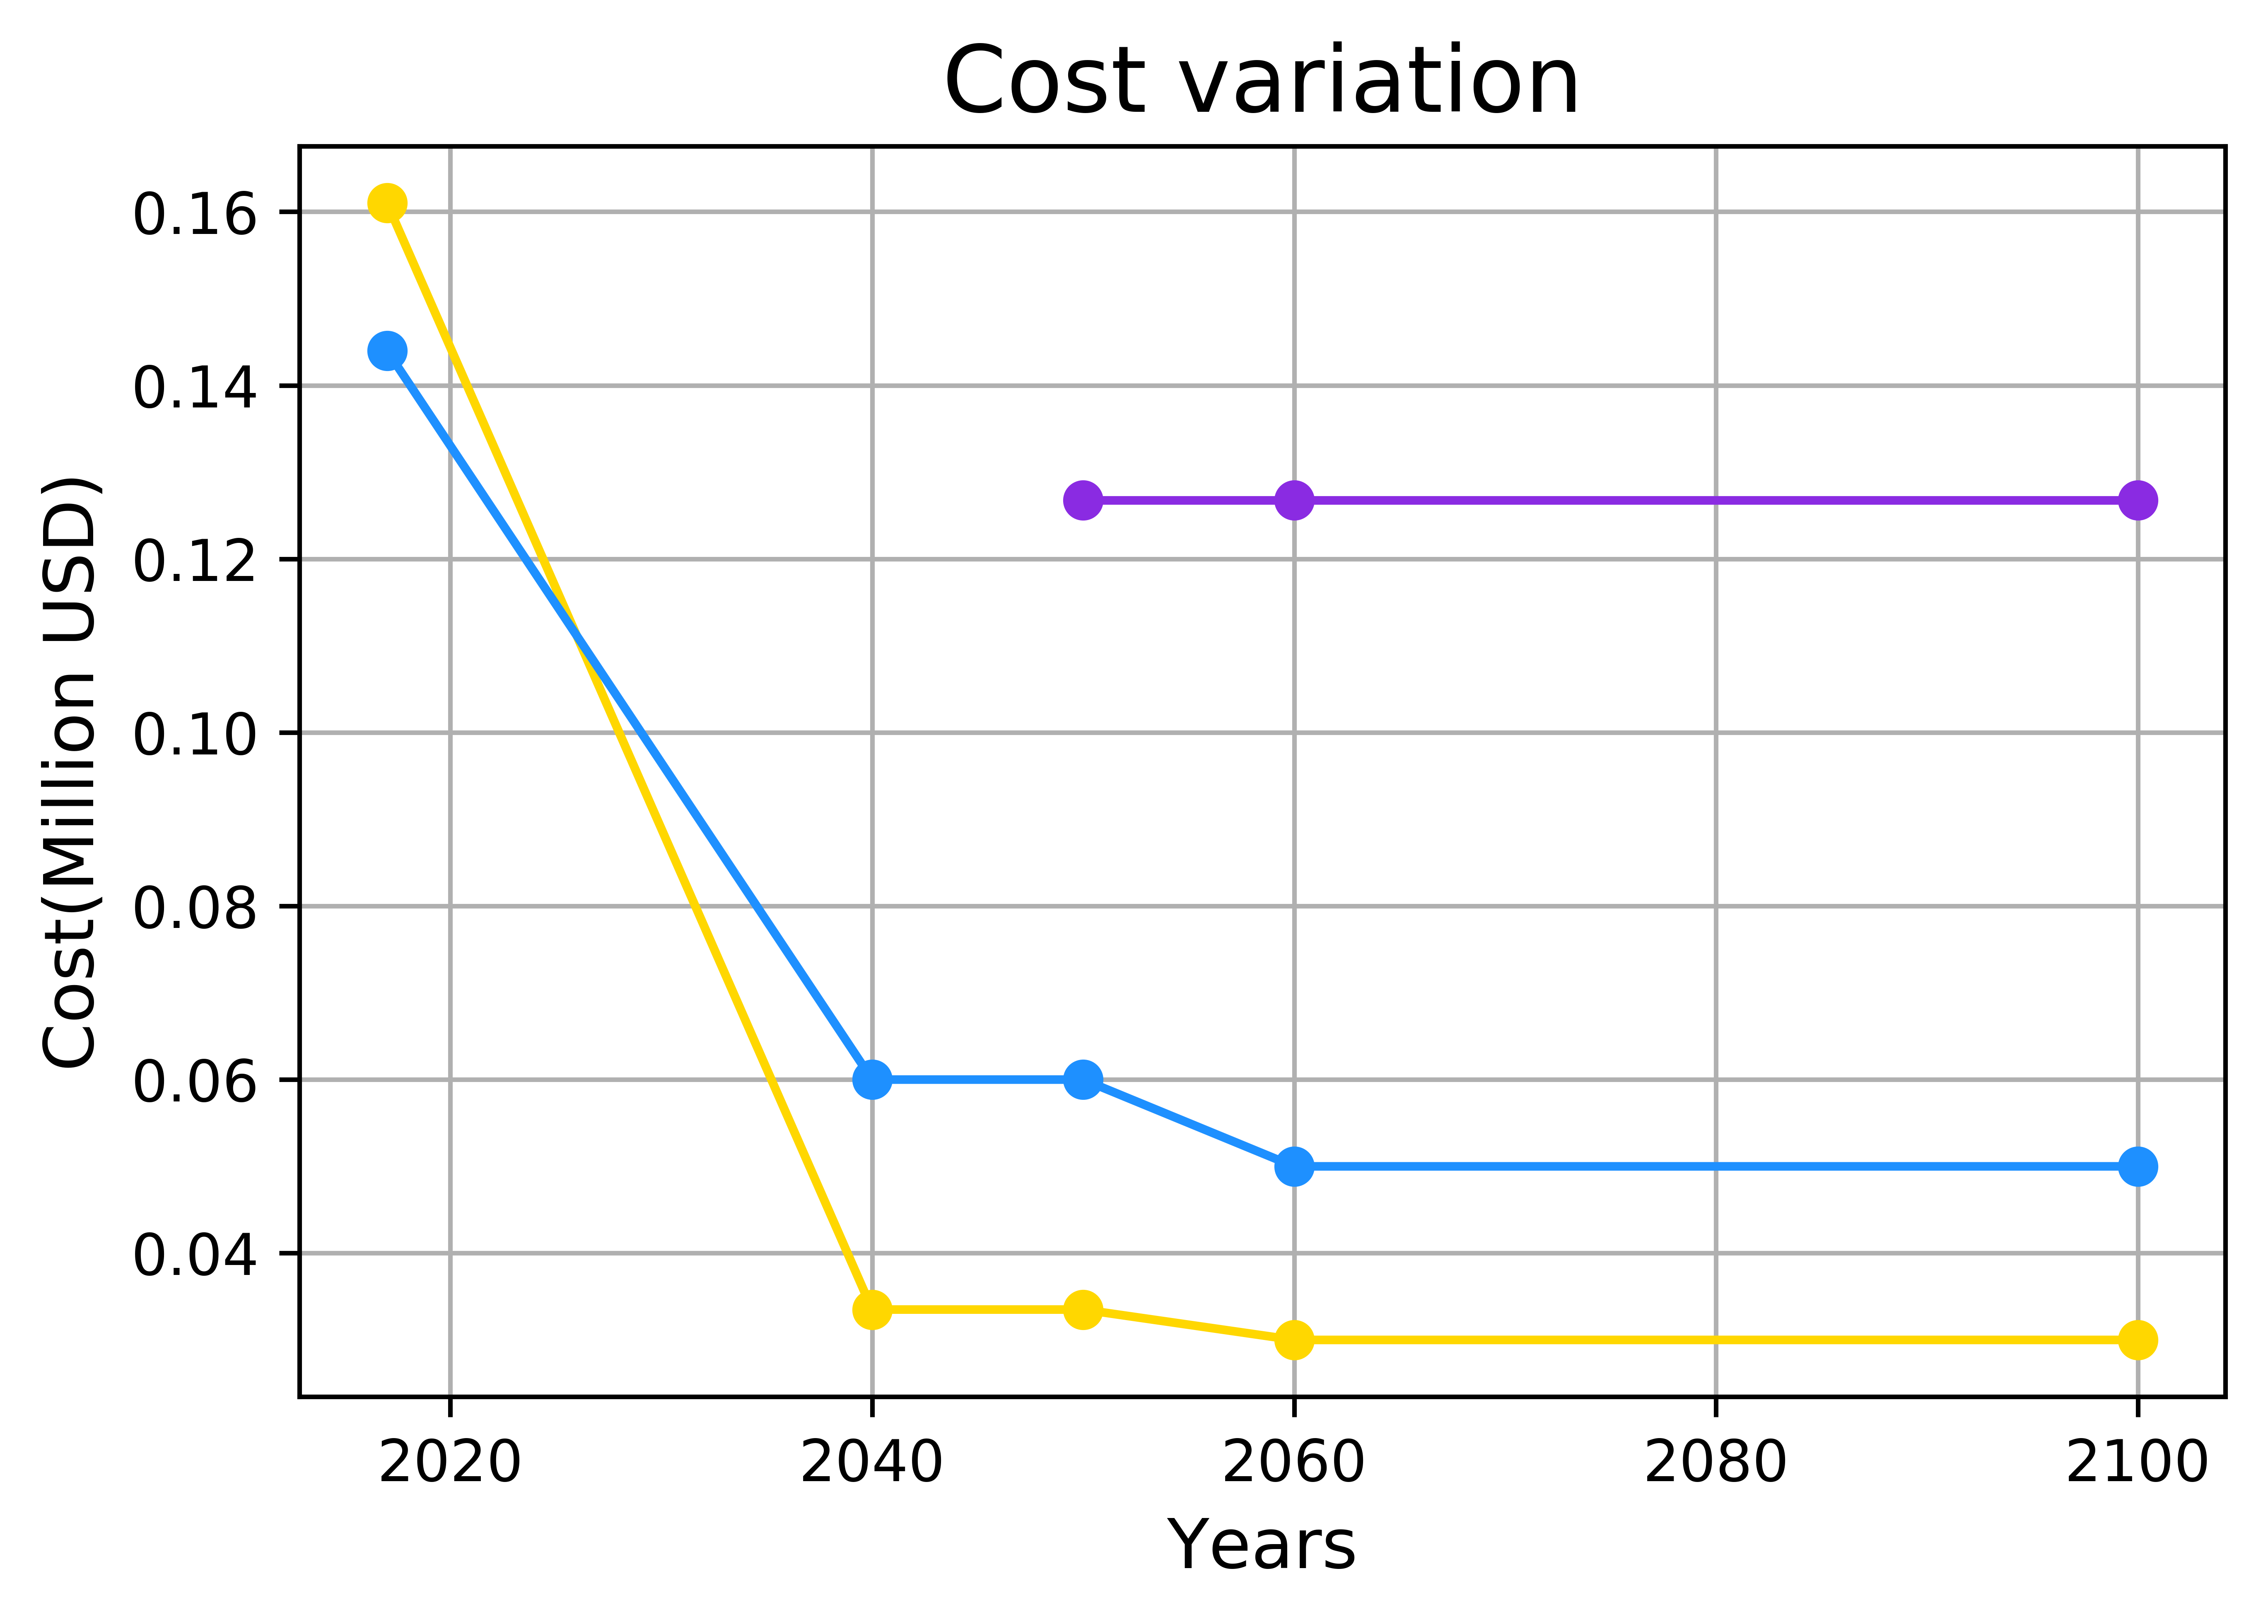
\includegraphics[scale=1.6]{cost}
\caption{Cost variation in solar, wind, and photocatalytic H$_2$ production.}
\label{cost}
\end{figure}
         \begin{alertblock}{Take Aways}
	\begin{itemize}
                \item Nuclear power is the cleanest and cheapest.
                                        
                \item Without nuclear and I$^2$CNER, solar and wind are deployed in a 1:2 ratio.
                
                \item H$_2$ and wind can meet I$^2$CNER targets without nuclear, at high cost.
                
                \item Highest impact so far: nuclear power, offshore wind, photocatalytic H$_2$, solar
	\end{itemize}
        \end{alertblock}
   


%--------------------------------------------------------
% PROJECT TIMELINE
%---------------------------------------------------------
\begin{block}{Limitations and Future work}
    \begin{itemize}
    
    \item Model focuses on \textbf{electricity supply sector}.
    
    \item Cost of fossil fuels, geothermal, hydropower, steam reforming and nuclear is constant.
        
    \item Emissions tied to energy production, not capacity installation.
    
    \item Annual timestep can't capture variation in wind, solar.    
    
    \item Capture realistic transitions and fluctuations in demand.
    
    \item Incorporation of more I$^2$CNER technologies.
    
    \item Sensitivity and cost analysis to maximize I$^2$CNER's impact.
    
    %\item Detailed cost analysis
    
    \item Add energy storage to supplement renewables and H$_2$. 
    
    \end{itemize}
\end{block}

\begin{block}{References}
        {\footnotesize\bibliographystyle{ieeetr} 
        \bibliography{2019-chaube-i2cner-poster}}
\end{block}

%----------------------------------------------------------------------------------------

%----------------------------------------------------------------------------------------
%	CONTACT INFORMATION
%----------------------------------------------------------------------------------------

\setbeamercolor{block alerted title}{fg=black,bg=norange} % Change the alert block title colors
\setbeamercolor{block alerted body}{fg=black,bg=white} % Change the alert block body colors

\begin{alertblock}{Contact Information}
\begin{itemize}
	\item Web: \href{arfc.github.io}{arfc.github.io}
	\item Email: \href{mailto:kdhuff@illinois.edu}{kdhuff@illinois.edu}
\end{itemize}

\end{alertblock}

%----------------------------------------------------------------------------------------
%	ACKNOWLEDGEMENTS
%----------------------------------------------------------------------------------------

\setbeamercolor{block title}{fg=norange,bg=white} % Change the block title color

\begin{block}{Acknowledgements}

This research is being performed using funding received
from the International Institute for Carbon Neutral Energy Research (I$^2$CNER) 
Initiative on Challenges in Energy Assessment and Energy Transitions at  the  
University of Illinois under Director Petros Sofronis.

%\vspace{10mm}
\begin{center}
\begin{tabular}{cccc}

\includegraphics[scale=0.7]{arfc_logo.png} & 
\includegraphics[scale=0.5]{wpi_logo.png} & 
\includegraphics[scale=0.1]{ku_logo.png} &
\includegraphics[scale=0.7]{i2cner_logo.png}
%
\includegraphics[width=\linewidth, height=0.1\textheight]{i2cner_logo.png}
\end{tabular}
\end{center}


\end{block}

\end{column} % End of the final column

\end{columns}
\end{frame} % End of the enclosing frame

\end{document}
